%%%%%%%%%%%%%%%%%%%%%%%%%%%%%%%%%%%%%%%%%%%%%%%%%%%%%%%%%%%%%%%%%%%%%%
% Template for a UBC-compliant dissertation
% At the minimum, you will need to change the information found
% after the "Document meta-data"
%
%!TEX TS-program = pdflatex
%!TEX encoding = UTF-8 Unicode

%% The ubcdiss class provides several options:
%%   fogscopy
%%       set parameters to exactly how FoGS specifies
%%         * single-sided
%%         * page-numbering starts from title page
%%         * the lists of figures and tables have each entry prefixed
%%           with 'Figure' or 'Table'
%%       This can be tested by `\iffogscopy ... \else ... \fi'
%%   10pt, 11pt, 12pt
%%       set default font size
%%   oneside, twoside
%%       whether to format for single-sided or double-sided printing
%%   balanced
%%       when double-sided, ensure page content is centred
%%       rather than slightly offset (the default)
%%   singlespacing, onehalfspacing, doublespacing
%%       set default inter-line text spacing; the ubcdiss class
%%       provides \textspacing to revert to this configured spacing
%%   draft
%%       disable more intensive processing, such as including
%%       graphics, etc.
%%

% For submission to FoGS
\documentclass[fogscopy,onehalfspacing,11pt]{ubcdiss}

% For your own copies (looks nicer)
% \documentclass[balanced,twoside,11pt]{ubcdiss}

%%%%%%%%%%%%%%%%%%%%%%%%%%%%%%%%%%%%%%%%%%%%%%%%%%%%%%%%%%%%%%%%%%%%%%
%%%%%%%%%%%%%%%%%%%%%%%%%%%%%%%%%%%%%%%%%%%%%%%%%%%%%%%%%%%%%%%%%%%%%%
%%
%% FONTS:
%% 
%% The defaults below configures Times Roman for the serif font,
%% Helvetica for the sans serif font, and Courier for the
%% typewriter-style font.  Configuring fonts can be time
%% consuming; we recommend skipping to END FONTS!
%% 
%% If you're feeling brave, have lots of time, and wish to use one
%% your platform's native fonts, see the commented out bits below for
%% XeTeX/XeLaTeX.  This is not for the faint at heart. 
%% (And shouldn't you be writing? :-)
%%

%% NFSS font specification (New Font Selection Scheme)
\usepackage{times,mathptmx,courier}
\usepackage[scaled=.92]{helvet}

%% Math or theory people may want to include the handy AMS macros
%\usepackage{amssymb}
%\usepackage{amsmath}
%\usepackage{amsfonts}

%% The pifont package provides access to the elements in the dingbat font.   
%% Use \ding{##} for a particular dingbat (see p7 of psnfss2e.pdf)
%%   Useful:
%%     51,52 different forms of a checkmark
%%     54,55,56 different forms of a cross (saltyre)
%%     172-181 are 1-10 in open circle (serif)
%%     182-191 are 1-10 black circle (serif)
%%     192-201 are 1-10 in open circle (sans serif)
%%     202-211 are 1-10 in black circle (sans serif)
%% \begin{dinglist}{##}\item... or dingautolist (which auto-increments)
%% to create a bullet list with the provided character.
\usepackage{pifont}

%%%%%%%%%%%%%%%%%%%%%%%%%%%%%%%%%%%%%%%%%%%%%%%%%%%%%%%%%%%%%%%%%%%%%%
%% Configure fonts for XeTeX / XeLaTeX using the fontspec package.
%% Be sure to check out the fontspec documentation.
%\usepackage{fontspec,xltxtra,xunicode}	% required
%\defaultfontfeatures{Mapping=tex-text}	% recommended
%% Minion Pro and Myriad Pro are shipped with some versions of
%% Adobe Reader.  Adobe representatives have commented that these
%% fonts can be used outside of Adobe Reader.
%\setromanfont[Numbers=OldStyle]{Minion Pro}
%\setsansfont[Numbers=OldStyle,Scale=MatchLowercase]{Myriad Pro}
%\setmonofont[Scale=MatchLowercase]{Andale Mono}

%% Other alternatives:
%\setromanfont[Mapping=tex-text]{Adobe Caslon}
%\setsansfont[Scale=MatchLowercase]{Gill Sans}
%\setsansfont[Scale=MatchLowercase,Mapping=tex-text]{Futura}
%\setmonofont[Scale=MatchLowercase]{Andale Mono}
%\newfontfamily{\SYM}[Scale=0.9]{Zapf Dingbats}
%% END FONTS
%%%%%%%%%%%%%%%%%%%%%%%%%%%%%%%%%%%%%%%%%%%%%%%%%%%%%%%%%%%%%%%%%%%%%%
%%%%%%%%%%%%%%%%%%%%%%%%%%%%%%%%%%%%%%%%%%%%%%%%%%%%%%%%%%%%%%%%%%%%%%



%%%%%%%%%%%%%%%%%%%%%%%%%%%%%%%%%%%%%%%%%%%%%%%%%%%%%%%%%%%%%%%%%%%%%%
%%%%%%%%%%%%%%%%%%%%%%%%%%%%%%%%%%%%%%%%%%%%%%%%%%%%%%%%%%%%%%%%%%%%%%
%%
%% Recommended packages
%%
\usepackage{checkend}	% better error messages on left-open environments
\usepackage{graphicx}	% for incorporating external images

%% booktabs: provides some special commands for typesetting tables as used
%% in excellent journals.  Ignore the examples in the Lamport book!
\usepackage{booktabs}

%% listings: useful support for including source code listings, with
%% optional special keyword formatting.  The \lstset{} causes
%% the text to be typeset in a smaller sans serif font, with
%% proportional spacing.
\usepackage{listings}
\lstset{basicstyle=\sffamily\scriptsize,showstringspaces=false,fontadjust}

%% The acronym package provides support for defining acronyms, providing
%% their expansion when first used, and building glossaries.  See the
%% example in glossary.tex and the example usage throughout the example
%% document.
%% NOTE: to use \MakeTextLowercase in the \acsfont command below,
%%   we *must* use the `nohyperlinks' option -- it causes errors with
%%   hyperref otherwise.  See Section 5.2 in the ``LaTeX 2e for Class
%%   and Package Writers Guide'' (clsguide.pdf) for details.
\usepackage[printonlyused,nohyperlinks]{acronym}
%% The ubcdiss.cls loads the `textcase' package which provides commands
%% for upper-casing and lower-casing text.  The following causes
%% the acronym package to typeset acronyms in small-caps
%% as recommended by Bringhurst.
\renewcommand{\acsfont}[1]{{\scshape \MakeTextLowercase{#1}}}

%% color: add support for expressing colour models.  Grey can be used
%% to great effect to emphasize other parts of a graphic or text.
%% For an excellent set of examples, see Tufte's "Visual Display of
%% Quantitative Information" or "Envisioning Information".
\usepackage{color}
\definecolor{greytext}{gray}{0.5}

%% comment: provides a new {comment} environment: all text inside the
%% environment is ignored.
%%   \begin{comment} ignored text ... \end{comment}
\usepackage{comment}

%% The natbib package provides more sophisticated citing commands
%% such as \citeauthor{} to provide the author names of a work,
%% \citet{} to produce an author-and-reference citation,
%% \citep{} to produce a parenthetical citation.
%% We use \citeeg{} to provide examples
\usepackage[numbers,sort&compress]{natbib}
\newcommand{\citeeg}[1]{\citep[e.g.,][]{#1}}

%% The titlesec package provides commands to vary how chapter and
%% section titles are typeset.  The following uses more compact
%% spacings above and below the title.  The titleformat that follow
%% ensure chapter/section titles are set in singlespace.
\usepackage[compact]{titlesec}
\titleformat*{\section}{\singlespacing\raggedright\bfseries\Large}
\titleformat*{\subsection}{\singlespacing\raggedright\bfseries\large}
\titleformat*{\subsubsection}{\singlespacing\raggedright\bfseries}
\titleformat*{\paragraph}{\singlespacing\raggedright\itshape}

%% The caption package provides support for varying how table and
%% figure captions are typeset.
\usepackage[format=hang,indention=-1cm,labelfont={bf},margin=1em]{caption}

%% url: for typesetting URLs and smart(er) hyphenation.
%% \url{http://...} 
\usepackage{url}
\urlstyle{sf}	% typeset urls in sans-serif


%%%%%%%%%%%%%%%%%%%%%%%%%%%%%%%%%%%%%%%%%%%%%%%%%%%%%%%%%%%%%%%%%%%%%%
%%%%%%%%%%%%%%%%%%%%%%%%%%%%%%%%%%%%%%%%%%%%%%%%%%%%%%%%%%%%%%%%%%%%%%
%%
%% Possibly useful packages: you may need to explicitly install
%% these from CTAN if they aren't part of your distribution;
%% teTeX seems to ship with a smaller base than MikTeX and MacTeX.
%%
%\usepackage{pdfpages}	% insert pages from other PDF files
%\usepackage{longtable}	% provide tables spanning multiple pages
%\usepackage{chngpage}	% support changing the page widths on demand
%\usepackage{tabularx}	% an enhanced tabular environment

%% enumitem: support pausing and resuming enumerate environments.
%\usepackage{enumitem}

%% rotating: provides two environments, sidewaystable and sidewaysfigure,
%% for typesetting tables and figures in landscape mode.  
%\usepackage{rotating}

%% subfig: provides for including subfigures within a figure,
%% and includes being able to separately reference the subfigures.
%\usepackage{subfig}

%% ragged2e: provides several new new commands \Centering, \RaggedLeft,
%% \RaggedRight and \justifying and new environments Center, FlushLeft,
%% FlushRight and justify, which set ragged text and are easily
%% configurable to allow hyphenation.
%\usepackage{ragged2e}

%% The ulem package provides a \sout{} for striking out text and
%% \xout for crossing out text.  The normalem and normalbf are
%% necessary as the package messes with the emphasis and bold fonts
%% otherwise.
%\usepackage[normalem,normalbf]{ulem}    % for \sout

%%%%%%%%%%%%%%%%%%%%%%%%%%%%%%%%%%%%%%%%%%%%%%%%%%%%%%%%%%%%%%%%%%%%%%
%% HYPERREF:
%% The hyperref package provides for embedding hyperlinks into your
%% document.  By default the table of contents, references, citations,
%% and footnotes are hyperlinked.
%%
%% Hyperref provides a very handy command for doing cross-references:
%% \autoref{}.  This is similar to \ref{} and \pageref{} except that
%% it automagically puts in the *type* of reference.  For example,
%% referencing a figure's label will put the text `Figure 3.4'.
%% And the text will be hyperlinked to the appropriate place in the
%% document.
%%
%% Generally hyperref should appear after most other packages

%% The following puts hyperlinks in very faint grey boxes.
%% The `pagebackref' causes the references in the bibliography to have
%% back-references to the citing page; `backref' puts the citing section
%% number.  See further below for other examples of using hyperref.
%% 2009/12/09: now use `linktocpage' (Jacek Kisynski): FoGS now prefers
%%   that the ToC, LoF, LoT place the hyperlink on the page number,
%%   rather than the entry text.
\usepackage[bookmarks,bookmarksnumbered,%
    citebordercolor={0.8 0.8 0.8},filebordercolor={0.8 0.8 0.8},%
    linkbordercolor={0.8 0.8 0.8},pagebordercolor={0.8 0.8 0.8},%
    urlbordercolor={0.8 0.8 0.8},%
    pagebackref,linktocpage%
    ]{hyperref}
%% The following change how the the back-references text is typeset in a
%% bibliography when `backref' or `pagebackref' are used
\renewcommand\backrefpagesname{\(\rightarrow\) pages}
\renewcommand\backref{\textcolor{greytext} \backrefpagesname\ }

%% The following uses most defaults, which causes hyperlinks to be
%% surrounded by colourful boxes; the colours are only visible in
%% PDFs and don't show up when printed:
%\usepackage[bookmarks,bookmarksnumbered]{hyperref}

%% The following disables the colourful boxes around hyperlinks.
%\usepackage[bookmarks,bookmarksnumbered,pdfborder={0 0 0}]{hyperref}

%% The following disables all hyperlinking, but still enabled use of
%% \autoref{}
%\usepackage[draft]{hyperref}

%% The following commands causes chapter and section references to
%% uppercase the part name.
\renewcommand{\chapterautorefname}{Chapter}
\renewcommand{\sectionautorefname}{Section}
\renewcommand{\subsectionautorefname}{Section}
\renewcommand{\subsubsectionautorefname}{Section}


%%%%%%%%%%%%%%%%%%%%%%%%%%%%%%%%%%%%%%%%%%%%%%%%%%%%%%%%%%%%%%%%%%%%%%
%%%%%%%%%%%%%%%%%%%%%%%%%%%%%%%%%%%%%%%%%%%%%%%%%%%%%%%%%%%%%%%%%%%%%%
%%
%% Some special settings that controls how text is typeset
%%
% \raggedbottom		% pages don't have to line up nicely on the last line
% \sloppy		% be a bit more relaxed in inter-word spacing
% \clubpenalty=10000	% try harder to avoid orphans
% \widowpenalty=10000	% try harder to avoid widows
% \tolerance=1000

%% And include some of our own useful macros
% This file provides examples of some useful macros for typesetting
% dissertations.  None of the macros defined here are necessary beyond
% for the template documentation, so feel free to change, remove, and add
% your own definitions.
%
% We recommend that you define macros to separate the semantics
% of the things you write from how they are presented.  For example,
% you'll see definitions below for a macro \file{}: by using
% \file{} consistently in the text, we can change how filenames
% are typeset simply by changing the definition of \file{} in
% this file.
% 
%% The following is a directive for TeXShop to indicate the main file
%%!TEX root = diss.tex

\newcommand{\NA}{\textsc{n/a}}	% for "not applicable"
\newcommand{\eg}{e.g.,\ }	% proper form of examples (\eg a, b, c)
\newcommand{\ie}{i.e.,\ }	% proper form for that is (\ie a, b, c)
\newcommand{\etal}{\emph{et al}}

% Some useful macros for typesetting terms.
\newcommand{\file}[1]{\texttt{#1}}
\newcommand{\class}[1]{\texttt{#1}}
\newcommand{\latexpackage}[1]{\href{http://www.ctan.org/macros/latex/contrib/#1}{\texttt{#1}}}
\newcommand{\latexmiscpackage}[1]{\href{http://www.ctan.org/macros/latex/contrib/misc/#1.sty}{\texttt{#1}}}
\newcommand{\env}[1]{\texttt{#1}}
\newcommand{\BibTeX}{Bib\TeX}

% Define a command \doi{} to typeset a digital object identifier (DOI).
% Note: if the following definition raise an error, then you likely
% have an ancient version of url.sty.  Either find a more recent version
% (3.1 or later work fine) and simply copy it into this directory,  or
% comment out the following two lines and uncomment the third.
\DeclareUrlCommand\DOI{}
\newcommand{\doi}[1]{\href{http://dx.doi.org/#1}{\DOI{doi:#1}}}
%\newcommand{\doi}[1]{\href{http://dx.doi.org/#1}{doi:#1}}

% Useful macro to reference an online document with a hyperlink
% as well with the URL explicitly listed in a footnote
% #1: the URL
% #2: the anchoring text
\newcommand{\webref}[2]{\href{#1}{#2}\footnote{\url{#1}}}

% epigraph is a nice environment for typesetting quotations
\makeatletter
\newenvironment{epigraph}{%
	\begin{flushright}
	\begin{minipage}{\columnwidth-0.75in}
	\begin{flushright}
	\@ifundefined{singlespacing}{}{\singlespacing}%
    }{
	\end{flushright}
	\end{minipage}
	\end{flushright}}
\makeatother

% \FIXME{} is a useful macro for noting things needing to be changed.
% The following definition will also output a warning to the console
\newcommand{\FIXME}[1]{\typeout{**FIXME** #1}\textbf{[FIXME: #1]}}

% END


%%%%%%%%%%%%%%%%%%%%%%%%%%%%%%%%%%%%%%%%%%%%%%%%%%%%%%%%%%%%%%%%%%%%%%
%%%%%%%%%%%%%%%%%%%%%%%%%%%%%%%%%%%%%%%%%%%%%%%%%%%%%%%%%%%%%%%%%%%%%%
%%
%% Document meta-data: be sure to also change the \hypersetup information
%%

\title{Playing Atari 2600 games by relational template selection}
%\subtitle{If you want a subtitle}

\author{Hai Feng Kao}
\previousdegree{M.Sc., National Taiwan University, 2006}
\previousdegree{B.Sc., National Taiwan University, 2004}

% What is this dissertation for?
\degreetitle{Master of Science}

\institution{The University Of British Columbia}
\campus{Vancouver}

\faculty{The Faculty of Graduate Studies}
\department{Computer Science}
\submissionmonth{April}
\submissionyear{2011}

%% hyperref package provides support for embedding meta-data in .PDF
%% files
\hypersetup{
  pdftitle={Relational Template Selection(DRAFT: \today)},
  pdfauthor={Hai Feng Kao},
  pdfkeywords={Relational Reinforcement Learning}
}

%%%%%%%%%%%%%%%%%%%%%%%%%%%%%%%%%%%%%%%%%%%%%%%%%%%%%%%%%%%%%%%%%%%%%%
%%%%%%%%%%%%%%%%%%%%%%%%%%%%%%%%%%%%%%%%%%%%%%%%%%%%%%%%%%%%%%%%%%%%%%
%% 
%% The document content
%%

%% LaTeX's \includeonly commands causes any uses of \include{} to only
%% include files that are in the list.  This is helpful to produce
%% subsets of your thesis (e.g., for committee members who want to see
%% the dissertation chapter by chapter).  It also saves time by 
%% avoiding reprocessing the entire file.
%\includeonly{intro,conclusions}
%\includeonly{discussion}

\begin{document}

%%%%%%%%%%%%%%%%%%%%%%%%%%%%%%%%%%%%%%%%%%%%%%%%%%
%% From Thesis Components: Tradtional Thesis
%% <http://www.grad.ubc.ca/students/thesis/index.asp?menu=003,000,000,000>

% Preliminary Pages (numbered in lower case Roman numerals)
%    1. Title page (mandatory)
\maketitle

%    2. Abstract (mandatory - maximum 350 words)
%% The following is a directive for TeXShop to indicate the main file
%%!TEX root = diss.tex

%Introduction
%RL->MDP, Q, SARSA, SMDP, 
%MAXQ (include the algorithm), hierarchical optimal vs recursive optimal, HORDQ, Relational,  Model-based RL (cite Peter Stone's Model based approach and a brief intro of it, include the algorithm)
%the problem of HO
%Optimal planning, model the differences
%scale to large problems
%The power of model-based RL and relational approach--> use a maze to illustrate this(model the difference)
%Linear SARSA
%Super Mario

%Motivation:
%1. scale to large problem with small number of samples

%chpater 2: 
%1. MaxQ

%chapter 3:
%1. The power of model based approach--> one wall sample and one pincecess can solve the whole maze problem
   %1.1. show the effectiveness
   %1.2. scaling up--> a noval biased model-based approach (show that it is the only way)
   %1.3. the necessity of biased approach
   %1.4. the choice between planning variable and not
   %1.5. wrong decision variable causes disater (decision)

%chapter 4:
%1. the three optimality ()
%2. Combined with hierarchical optimal RL
%3. why we need leaf cover
%4. the convergence for online approach
%5. the offiline one
%6. Respect the hierarchy

%chpater 5 scaling it up
%1. Better generalization: relational rl
%1.1. the power of model the difference
%2. Reduce training time: transfer learning
%3. case study: Super Mario

%chapter 6 future work
%1. make it hierarchical optimal (add only put down to get passenger subtask in taxi domain)
%2. A general way to combine any approximated model-based approach and can still achieve optimality
\chapter{Abstract}

Model-based reinforcement learning methods make efficient use of samples by
building a model of the environment and planning with it. Compared to
model-free methods, they usually take fewer samples to converge to the optimal
policy. Despite that efficiency, model-based methods may not learn the optimal
policy due to structural modeling assumptions. In this thesis, we show that by
combining model-based methods with hierarchically optimal recursive Q-learning (HORDQ)
under a hierarchical reinforcement learning framework, the proposed approach
learns the optimal policy even when the assumptions of the model are not
satisfied.
%we propose a simple approach that assumes most of the variables are static
%during the planning process and focuses on modeling the few dynamic variables.

% Embed version information inline -- you should remove this from your
% dissertation
\vfill
\begin{center}
\begin{sf}
\fbox{Revision: ubcdiss.cls r27
}
\end{sf}
\end{center}

\cleardoublepage

%    3. Table of contents (mandatory - list all items in the preliminary pages
%    starting with the abstract, followed by chapter headings and
%    subheadings, bibliographies and appendices)
\tableofcontents
\cleardoublepage	% required by tocloft package

%    4. List of tables (mandatory if thesis has tables)
\listoftables
\cleardoublepage	% required by tocloft package

%    5. List of figures (mandatory if thesis has figures)
\listoffigures
\cleardoublepage	% required by tocloft package

%    6. List of illustrations (mandatory if thesis has illustrations)
%    7. Lists of symbols, abbreviations or other (optional)

%    8. Glossary (optional)
%% The following is a directive for TeXShop to indicate the main file
%%!TEX root = diss.tex

\chapter{Glossary}

This glossary uses the handy \latexpackage{acroynym} package to automatically
maintain the glossary.  It uses the package's \texttt{printonlyused}
option to include only those acronyms explicitly referenced in the
\LaTeX\ source.

% use \acrodef to define an acronym, but no listing
\acrodef{UI}{user interface}
\acrodef{UBC}{University of British Columbia}

% The acronym environment will typeset only those acronyms that were
% *actually used* in the course of the document
\begin{acronym}[ANOVA]
\acro{ANOVA}[ANOVA]{Analysis of Variance\acroextra{, a set of
  statistical techniques to identify sources of variability between groups}}
\acro{API}{application programming interface}
\acro{CTAN}{\acroextra{The }Common \TeX\ Archive Network}
\acro{DOI}{Document Object Identifier\acroextra{ (see
    \url{http://doi.org})}}
\acro{FoGS}[FoGS]{The Faculty of Graduate Studies}
\acro{PDF}{Portable Document Format}
\acro{RCS}[RCS]{Revision control system\acroextra{, a software
    tool for tracking changes to a set of files}}
\acro{TLX}[TLX]{Task Load Index\acroextra{, an instrument for gauging
  the subjective mental workload experienced by a human in performing
  a task}}
\acro{UML}{Unified Modelling Language\acroextra{, a visual language
    for modelling the structure of software artefacts}}
\acro{URL}{Unique Resource Locator\acroextra{, used to describe a
    means for obtaining some resource on the world wide web}}
\acro{W3C}[W3C]{\acroextra{the }World Wide Web Consortium\acroextra{,
    the standards body for web technologies}}
\acro{XML}{Extensible Markup Language}
\end{acronym}

% You can also use \newacro{}{} to only define acronyms
% but without explictly creating a glossary
% 
% \newacro{ANOVA}[ANOVA]{Analysis of Variance\acroextra{, a set of
%   statistical techniques to identify sources of variability between groups.}}
% \newacro{API}[API]{application programming interface}
% \newacro{GOMS}[GOMS]{Goals, Operators, Methods, and Selection\acroextra{,
%   a framework for usability analysis.}}
% \newacro{TLX}[TLX]{Task Load Index\acroextra{, an instrument for gauging
%   the subjective mental workload experienced by a human in performing
%   a task.}}
% \newacro{UI}[UI]{user interface}
% \newacro{UML}[UML]{Unified Modelling Language}
% \newacro{W3C}[W3C]{World Wide Web Consortium}
% \newacro{XML}[XML]{Extensible Markup Language}
	% always input, since other macros may rely on it

\textspacing		% begin one-half or double spacing

%    9. Preface (optional)
%   10. Acknowledgements (optional)
%% The following is a directive for TeXShop to indicate the main file
%%!TEX root = diss.tex

\chapter{Acknowledgments}

I am very fortunate to have the opportunity to study and do research in
University of British Columbia. I am most grateful to my supervisor, Alan Mackworth.
When I proposed the idea of developing a generic game AI for video games, he
accepted and allowed me to work on a problem which I am really passionate about.
Besides, I would like to thank David Buchman, John Chia and Bruno Norberto da Silva
for sharing their knowledge and expertise in reinforcement learning.
%Without his encouragement and kindness, I would have gave up this idea long before.
I would also like to thank Tzu-Kuo Huang for sharing
the new research works done at CMU. One of the works actually inspired
the idea of this thesis.
A special thank goes to Prof. Poole, who gave me many precious ideas to make this
thesis better.
And most importantly, I would like to thank my parents, who support
me whenever I need it. Without them, it is impossible to finish this work.
%Thank those people who helped you. 

%Don't forget your parents or loved ones.

%You may wish to acknowledge your funding sources.

%I have been very fortunate to have an enjoyable and fruitful learning experience here in
%University of Alberta, and for this I am most grateful to my supervisor, Michael Bowling.
%He has provided me with the opportunity to work on a research topic that I am truly
%passionate about, given me enough academic freedom to experiment and learn on my own,
%and yet he has always been there to guide me when I was lost and confused.
%I am very thankful to my fellow graduate students who have generously and patiently
%shared their knowledge and expertise and have been instrumental for the completion of this
%thesis. In particular, I would like to thank Marc Lanctot and Chris Rayner for sharing their
%knowledge and getting me started with the Atari 2600 hardware and the emulation tools,
%Mohammad Shaei for sharing his insights on the concepts behind the UCT algorithm,
%and Michael Johanson for oering his expertise on running batch simulations on computer
%clusters. Our late night discussions with Amir-Massoud Farahmand have been some of the
%best learning experiences I have had through the last two years. I am very grateful to him,
%who has been both an inspiring colleague and a good friend.
%I am indebted to the team behind Stella, the Atari 2600 emulator, for releasing their
%work as open-source and allowing me to build my toolset on top of their code. I would
%also like to thank Richard Sutton and the RLAI group for releasing the source code of their
%Tile-Coding and Sarsa() implementations. I hope that releasing my own code base as
%open-source will be similarly benecial to other researchers and hobbyists.

%I would like to thank my supervisor, Michiel van de Panne, for his continuous
%support, guidance, and his willingness to let me explore the research tangents
%that made my time here so enjoyable. Michiel's joyful excitement about the
%eld is infectious, and I will cherish the times we spent reverse-engineering
%the human and animal motor system. The insights I gained through our
%discussions about academia have been particularly helpful and shaped me
%as a researcher.
%I am also thankful to Nando de Freitas for contributing ideas to this project,
%and for helping me with this thesis. I had the opportunity to closely interact
%with Nando on many projects and endeavors over the last two years, and
%his support, excitement, and can-do attitude have been very helpful and
%inspiring.
%I would also like to extend my thanks to David Lowe, Bob Woodham, and
%Kevin Murphy, all of whom I've come to know and admire over the last two
%years. I also had the pleasure of working with Steve Wolfman and Kimberly
%Voll as a TA on several occasions, and I am thankful to have witnessed their
%inspiring dedication to teaching.
%My thanks go to my bullpen mates and lab mates Paul Vanetti, John Chia,
%Byron Knoll, Stelian Coros, Philippe Beaudoin, Ben Jones, and many others
%who I don't have enough space to name for contributing to a pleasant, fun
%working atmosphere and oering healthy distractions from work.
%I wish to thank my sister for her unconditional support, and my parents,
%who sacriced to bring us to Canada and made it possible for me to pursue
%my dreams.
%Last but not least, I wish to thank Shelly, for giving me something to look
%forward to every day.

%I thank my advisor Alan Mackworth for being extremely supportive, friendly and
%amazingly open to very different research ideas. It is incredible how you manage to
%keep me on track without restricting the paths I choose to follow. Your generosity
%and helpfulness are a great lesson that I hope I can replicate one day with my own
%students. You are an idol.
%I’m grateful for all my LCI colleagues, for the stimulating environment and
%support. I learned a lot from many of you. A special note goes to Prof Giuseppe
%Carenini who helped me with my PhD application and 
%All my family in Brazil, for all the emails, phone calls, thoughts. Thanks for
%all your patience, care, support. And I’m trying hard to find the time to go back
%and see you all again.
%ma femme. Nao sei se devo repetir os votos ou se
%referencio minhas teses de graduacao e mestrado. Em todo caso, Helena fica aqui
%registrada como a motivacao e inspiracao deste e de todo meu trabalho.



%   11. Dedication (optional)

% Body of Thesis (not all sections may apply)
\mainmatter

\acresetall	% reset all acronyms used so far

%    1. Introduction
%% The following is a directive for TeXShop to indicate the main file
%%!TEX root = diss.tex

\chapter{Introduction}
\label{ch:intro}

\section{Problem Statement}
The objective of this project is to build a software which can play a wide range 
of video games. To achieve this goal, the software shall not possess any game-specific 
information. Besides, the software shall be able to play the games in a non-intrusive approach.
That is, the software shall be able to extract the necessary information 
from the screenshot of the games and control the games from standard input devices such as keyboard.
Since most of video games use graphical display as the primary interface, this requirement allows
the software to be applied to different video games.

\section{Why video games?}
Over the past decade, substantial research has been conducted to teach computer play classic strategy games such
as Deep Thought\cite{DeepBlue}, TD-Gammon\cite{Gammon}, and GO\cite{Go}.
On the other hand, little research has been made\cite{FPS}\cite{Mario} to extend the effort to other genres of video games.
The genres of video games include not only classic strategy games, but also action, first-person shooter, role-player, adventure, simulation, etc.
Video games introduce a new challenge to the AI community.

The challenge includes:
\begin{itemize}{}

\item A generic algorithm which can adapt to different types of games:
Following the paradigm of \cite{GGP} and \cite{Yavar}, the objective is not to design a good AI for
a specific game. Instead, the objective is to design a good and generic AI to play different games successfully.

\item Large but highly structured states:
For a 256 color video game with resolution $640 \times 480$, it has $256^(640 \times 480)$ states.
The number states are too big to be tractable. However, a video game often consists of small number of objects.
If we can figure out a way to represent the relationship of these objects, the number of states
can be reduced.

\item Dynamic number of agents:
Unlike classic strategy games, the number of agents in video games is highly dynamic.
The number of agents may increase over time and decrease if killed.
It is a challenge which doesn't exist in classic strategy games.
\end{itemize}

Video games can be viewed as a abstract representation of the real world. Often can we find the 
correspondence between such an artificial world to a real-world problem\cite{KeepAway}.
Focusing on Video games allows us to attack a real-world problem without tackling unnecessary details, while maintaining sufficient 
level of abstraction. In addition, video games are well-understood and customizable environments. 
It allows us to test an AI algorithm and justify if the result is correct\cite{Yavar}.

Another possible application is the AI of video games.
Nowadays, the AI engineers usually need to craft the behavior of AI by hand. 
The process are time-consuming and the hard-coded behavior would produce unrealistic AI behavior.
If we can design a generic agent and let it act reactively with the environment, it can produce 
more various and unpredictable behaviors.

\section{Why applying computer vision to video games?}

The reason behind is the reality that most of the video games do not have source codes which are publicly available.
If a researcher needs to test his algorithm on Super Mario Bros., all he can do is to apply it on Infinite Mario Bros.,
which is an open source clone of original Super Mario Bros. He cannot test his algorithm on Mario Bros. 1 or 2, which are available
on binary format. If a researcher does not have source codes, he cannot extract the game states like the location
of Koopa Troopas which are mandatory for any AI algorithm to work. 

Using computer vision techniques to extract the information from the game screen is a way to solve this problem.
Because most of the video games uses graphics as the primary interface to interact with the player, it contains
the necessary information for the player to play. The use of computer vision allows us to test the algorithm
non-intrusively, without the effort to hack the game engine or reimplement the game.

Besides, the vision allows a more generic way for a computer to play a video game. It creates 
new applications which cannot be done by intrusive approaches.

\begin{itemize}{}
\item Non-intrusive and generic AI:
Have you ever played a good game with poor AI? Can you change it with a better one?
Without the source codes of the game or the engine support, the answer is usually "No".
Nevertheless, if we could design a software which can learn to play any video game, 
the answer can be changed to "Yes". The non-intrusive and generic agents can be 
applied to any video games with/without the support from the game company.

\item Modding: 
Game modding becomes popular in recent years \cite{Modding}. 
Modding allows users to customize the video games to suite their personal tastes.
The modding usually includes the introduce new content, modification of original one, or remove the unsatisfactory elements.
The process can be done by the support of game development kit released by the game company.
It can also be done without the support from the game company. However, the modders need to hack the game engine,
decode the data format and implement their own development kit. 
The process can be time-consuming and tedious.
If we could automate the process by having a software which can 
traverse the game and extract the in-game elements for us, it could save a lot of time.

\end{itemize}

%\chapter{Related Work}
%\label{ch:Related}
\section{Related Work}

There are several works which address how to design a good AI for certain type of video games.
McPartland et al. proposed a approach to allow bots in First-Person Shooter (FPS)
games to learn how to navigate the maze and handle combat \cite{FPS}. M. Smith et al. proposed a coordination 
framework to allow the bots to adapt to different strategy by reinforcement learning \cite{FPS_TEAM}. 
Michael et al. applied a Monte Carlo planning approach for Real-Time Strategy (RTS) gmaes to 
the Rush-the-Flag game \cite{RTS}. Ponsen et al. proposed hierarchical relational learning to learn how to play
the Battle of Survival game \cite{HRRL}. For arcade-style games, \cite{Mario} uses a RL agent to learn
how to play Infinite Mario Bro. Driessens et al. proposed a relational RL to learn how to play the Digger
game. In \cite{OO}, a object-oriented representation is proposed to play pitfall.

Previous works rely on the intrusive approach to provide the states of games for the agents to play.
The agents need to know the information such as the number of objects, the types of objects,
or the health level of players to play the games. The intrusive approach makes it difficult to generalize
to a large number of video games. And the game-specific representation prevents these approaches
to be applied to arbitrary video games.

With the objective to play general video games, our work is most related to 
General Game Playing\cite{GGP} (GGP) and Playing Atari 2600 \cite{Yavar}. 
The objective of GGP is to develop a software agent which can play unspecific games if the rules
are given. Our work follows the same objective. However, due to the complexity of video games, 
it is not clear that how to precisely describe the rules of video games.

Y. Naddaf\cite{Yavar} proposed A.L.E. (Atari 2600 Learning Environment) as the platform to test AI algorithms.
A.L.E. supports fast emulation and generic interface. Fast emulation allows the emulator to run 
games without rendering or sound generation. It can increase the speed in the learning phase.
The generic interface provides AI agents the screenshot and scores in games. It allows us
to build the agents in a game independent way.

Our work is built on A.L.E. However, our work differs from \cite{Yavar} in the following perspective:

\begin{itemize}{}
\item Our work features object-based representation. We argue that objects are the fundamental elements
in video games. The representation allows the agent to develop appropriate policy against specific 
objects. And it also enables the possibility to reuse the knowledge in different stages.
\end{itemize}

\chapter{Reinforcement Learning}
\label{ch:RL}
The objective of reinforcement learning algorithm is to build an learning agent. The learning agent will take
actions based on the current state. In the beginning, the agent does not know anything about 
the environment, therefore the agent has to choose the first action randomly. After the environment
receives the action, it will provide a reward to the agent as a feedback. The reward can be either
positive or negative.

The agent adjusts the value function to maximize the expected reward in the future.
The value function represent the expected reward when the agent takes certain action in the current
state, and it is used to estimate the "quality" of an action. The initial value of value function is 
usually 0, but it is possible to set it to some high enough value to encourage exploration.
It is important to evaluate the value function 
correctly. If some actions with low expected reward are estimated as high, it degrades the
performance of agent.

The agent can select an action which leads to the highest value of value function. However, 
this strategy does not allow the agent to explore the states which are not visited before.
A better approach is to use $\epsilon$-greedy method. The method allows the agent to abandon the
best action and choose
a random action with a very small probability $\epsilon$. The higher the probability, the more
likely that the agent would explore the new actions. However, if the exploration probability 
is too high, it will increase the time to converge.

After the agent takes an action, the environment will provide a reward and a state to the
agent. The agent then decides an new action for the new state. After several iterations
, the agent will learn a correspondence between the action and state. The correspondence is called 
"policy". 

\section{Temporal Difference}
\label{sec:TD}
There are 3 types of reinforcement learning algorithms -- dynamic programming(DP), Monte Carlo 
methods, and temporal-difference (TD). Dynamic programming can compute the optimal policy, but it 
requires a precise model of the environment. In most of the cases, the environment
is too complex to be modeled precisely, and it is not easy to get the complete information about
the environment. On the other hand, it is usually possible to use Monte Carlo method to sample the environment to
get the partial information. 
Like Monte Carlo method, TD uses sampling, therefore it does not require the 
complete model of the environment. TD method is a bootstrapping method, similar to the dynamic 
programming approach, it updates the new value function based on the previous one.

The equation to compute the value function in TD:
\begin{displaymath}
   V(S_t) \leftarrow V(S_t) + \alpha [r_{t+1} + \gamma V(S_{t+1}) - V(S_t)],
\end{displaymath}

where $V(s_t)$ is the value function of the state $s_t$. $V(s_t)$ is the expected reward when
the agent reaches the state $s_t$. $r_{t+1}$ is the reward given to the agent when it chooses
the action at state $s_t$.

\section{SARSA}
\label{sec:SARSA}
SARSA is a on-policy TD approach. On-policy indicates that it learns from the current policy.
Different from other TD approaches, SARSA updates the Q value of the current state-action from the next state-action.
The Q value is updated by:
\begin{displaymath}
    Q(s_t, a_t) \leftarrow Q(s_t, a_t) + \alpha [r_{t+1} + \gamma Q(s_{t+1}, a_{t+1})-Q(s_t, a_t)],
\end{displaymath}
where $Q(s, a)$ is the value function for state-pair, and it is the expected reward when the agent takes
the action $a$ at the state $s$. $\alpha$ is step-wise, which controls the learning rate. 
$\gamma$ is the discount factor.


\begin{center}
\begin{tabular}{@{}lp{6cm}@{}}
\hline
Algorithm: SARSA\\
\hline
Initialize $Q(s, a)$ arbitrarily\\
Repeat (for each episode)\\
\ \ \ \ \ \ Initialize $s$\\
\ \ \ \ \ \ Choose $a$ based on $s$ using policy derived from $Q$ (e.g., $\epsilon$-greedy method)\\
\ \ \ \ \ \ Repeat (for each step of episode):\\
\ \ \ \ \ \ \ \ \ \ \ \ Take action $a$, obtain reward $r$ and next state $s'$ from the environment\\
\ \ \ \ \ \ \ \ \ \ \ \ Choose $a'$ based on $s'$ using policy derived from $Q$ (e.g., $\epsilon$-greedy method)\\
\ \ \ \ \ \ \ \ \ \ \ \ $Q(s, a) \leftarrow Q(s, a) + \alpha [r + \gamma Q(s', a')-Q(s, a)]$\\
\ \ \ \ \ \ \ \ \ \ \ \ $s \leftarrow s'$\\
\ \ \ \ \ \ \ \ \ \ \ \ $a \leftarrow a'$\\
\ \ \ \ \ \ Until $s$ is terminal\\
\hline  
\end{tabular}
\end{center}

\section{Q-Learning}
\label{sec:Q-Learning}
    Q-Learning is an off-policy TD approach. Compared to SARSA, Q-Learning updates
the Q value by the highest value of the next possible state-action, rather than the 
next state-action executed by the agent.  
The Q value is updated by:
\begin{displaymath}
   Q(s_t, a_t) \leftarrow Q(s_t, a_t) + \alpha [r_{t+1}+\gamma \max_a Q(s_{t+1},a)-Q(s_t,a_t)],
\end{displaymath}

where $\max_a Q(s_{t+1},a)$ is the highest value of the next possible state-action. 


\begin{center}
\begin{tabular}{@{}lp{6cm}@{}}
\hline
Algorithm: Q-Learning\\
\hline
Initialize $Q(s, a)$ arbitrarily\\
Repeat (for each episode)\\
\ \ \ \ \ \ Initialize $s$\\
\ \ \ \ \ \ Repeat (for each step of episode):\\
\ \ \ \ \ \ \ \ \ \ \ \ Choose $a$ based on $s$ using policy derived from $Q$ (e.g., $\epsilon$-greedy method)\\
\ \ \ \ \ \ \ \ \ \ \ \ Take action $a$, obtain reward $r$ and next state $s'$ from the environment\\
\ \ \ \ \ \ \ \ \ \ \ \ $Q(s, a) \leftarrow Q(s, a) + \alpha [r + \gamma max_{a'} Q(s', a')-Q(s, a)]$\\
\ \ \ \ \ \ \ \ \ \ \ \ $s \leftarrow s'$\\
\ \ \ \ \ \ Until $s$ is terminal\\
\hline  
\end{tabular}
\end{center}

\section{minmax Q-Learning}
\label{sec:minmax}

    In two player zero-sum game, it's reasonable to take the action of the opponent into consideration.
In minmax Q-learning, the Q value is a function of state, the action of player, and the action of opponent.
The Q value is updated by:
\begin{displaymath}
    Q(s_t, a_t, o_t) \leftarrow Q(s_t, a_t, o_t) + \alpha [r_{t+1}+\gamma\max_a min_o Q(s_{t+1}, a, o)-Q(s_t, a_t, o_t)],
\end{displaymath}

\begin{center}
\begin{tabular}{@{}lp{6cm}@{}}
\hline
Algorithm: minmax Q-learning\\
\hline
\ \ \ Initialize: $Q(s, a, o) \leftarrow 1, V(s) \leftarrow 1$
\ \ \ Repeat (for each episode)\\
\ \ \ \ \ \ Initialize $s$\\
\ \ \ \ \ \ Repeat (for each step of episode):\\
\ \ \ \ \ \ \ \ \ \ \ \ Choose $a$ based on $s$ using policy derived from $Q$ (e.g., $\epsilon$-greedy method)\\
\ \ \ \ \ \ \ \ \ \ \ \ Take action $a$, obtain opponent action $o$, reward $r$ and next state $s'$ from the environment\\
\ \ \ \ \ \ \ \ \ \ \ \ $Q(s, a, o) \leftarrow Q(s, a, o) + \alpha [r + \gamma max_{a'} min_{o'} Q(s', a', o')-Q(s, a, o)]$\\
\ \ \ \ \ \ \ \ \ \ \ \ $s \leftarrow s'$\\
\hline  
\end{tabular}
\end{center}


\chapter{Relational Learning}

Dynamic number of objects
No fixed representation
Dependency with samples. (intrinsic to reinforcement learning, since consective states has similar
Q-value, there are not independent all)

Video games involves objects: things like monsters, treasures, or princess.
But the most current machine learning algorithms requires the world to be represented 
by a vector of attributes. The vector representation has several drawbacks when applied to objects.


The vector representation is ordered. However, it's not clear how to assign a fixed for the objects.

The length of vector representation is fixed. However, the number of objects might vary.

The relationship between objects are lost in the vector representation. 

Motivation
Consider a typical questionanswering task on the
web 	BernersLee et al������  Fensel et al������ 
������
which might involve accessing and integrating semi
structured information from the web to answer a com
plex query������ eg������ nd a graduate school on the west
coast that has aordable housing������ multiple faculty and
funded research in Articial Intelligence Even if the
query is posed in a formal query language������ answer
ing it requires several skills such as query planning������
optimization������ information extraction������ and information
integration in a relational language Or consider what
is involved in learning to cook a meal While certainly
not an exhaustive list������ one needs to reason about peo
ples tastes and preferences������ ones own knowledge of
recipes and skills������ availability of ingredients������ their lo
cations������ and procedures to access them������ the capacities
of utensils and cooking ranges������ and the eects of dif
ferent proportions of ingredients������ of cooking temper
atures������ and of dierent kinds of cooking processes on
the taste and quality of the nal product
It is easy to pose both of these problems as reinforce
ment learning problems In both tasks������ we might pe
nalize the system for the time spent and other costs������
and reward it for the quality of the nal product
What is problematic������ however������ is that the structure
of the web and the reasoning involved in the cooking
task are most naturally represented using relational
representations This poses several challenges to the
success of RL in these domains
Function Approximation������ The valuefunction ap
proximation typically used in RL������ eg������ neural net
works or regression trees������ does not generalize well
when applied to relational domains This is partly
because these representations are illsuited to the
task of representing relational knowledge When
they are successful������ they require a careful choice of
propositional features or basis functions which are
handcrafted specically to a particular task at
hand Designing functionapproximation schemes
that exploit relational structure when present is a
critical challenge
Generalization across Objects������ RL methods that
do not explicitly represent objects and relation
ships between them are fundamentally limited in
their ability to transfer learning about one object
to similar related objects Critical challenges here
are identifying classes of objects that are to be
considered similar������ across which such general
ization is justied������ and identifying and represent
ing knowledge suitable for transfer
Transfer across Tasks������ RL programs are usually
tested on a single task and do not exhibit transfer
of knowledge across tasks Each task in a given
domain������ eg������ each query in information retrieval������
may look quite dierent when formulated propo
sitionally������ and thus may require separate training
to learn to answer it Relational representations
facilitate formulating broad collections of related
tasks as a single domain������ yielding natural gener
alization between these related tasks
Runtime Planning and Reasoning������ In most re
inforcement learning work������ there is no deliberate
planning and reasoning at runtime It is tac
itly assumed that either all planning occurs of
ine or the system relies completely on explo
ration and learning to construct good plans������ re
ducing the runtime execution to reactive behav
ior However������ complex dynamic domains require
both deliberation and reactivity������ as is demon
strated by successful gameplaying programs It
appears that the approximate nature of the value
function demands a more rened search at the run
time to compensate for its errors Reasoning may
also be important in constructing new features for
an improved valuefunction approximation
Prior Knowledge������ RL deemphasizes the role of
prior knowledge in learning and reasoning������ thus
relying on trial and error learning which can be
very ine
cient and often does not scale to more
complex tasks such as the above
Relational reinforcement learning 	RRL
 seeks to ad
dress all the above problems by generalizing RL to re
lationally represented states and actions In fact������ both
reinforcement learning and relational learning have a
long history The study of reinforcement learning be
gan with Samuels pioneering  work on checkers
	Samuel������ 
 Work on relational learning started
with Winstons work on blocks world learning 	Win
ston������ 
 In recent times������ relational learning is stud
ied under dierent names������ including inductive logic
programming������ relational data mining and probabilis
tic relational modeling Reinforcement learning is also
studied under multiple guises of which neurodynamic
programming and decision theoretic planning are the
most recognizable

%\section{Object-Oriented Relational Reinforcement Learning}
\section{Relational Markov Decision Processes}

Following the definition in \cite{RelationalMDP}, we define 
a relational MDP as follows:

Definition: Relational Markov decision process is formalized as a tuple $<C, S, O, D, A, T, R>$, where
\begin{itemize}{}
\item $C$ is a set of object classes $C={C_1, \dots, C_c}$. Each
class is associated with a set of state variables $S[C]={C.S_1, \dots, C.S_k}
    \item 
\end{itemize}
the system dynamics and rewards
at the level of a template for a task domain. Given a particular
environment within that domain, it defines a specific MDP
instantiated for that environment. The domain is specified by a schema,
which specifies a set of object classes $C = fC1; : : : ;Ccg. Each class
C is also associated with a set of state variables S[C] =
fC:S1; : : : ;C:Skg, which describe the state of an object in
that class. Each state variable C:S has a domain of possible
values Dom[C:S]. We define SC to be the set of possible
states for an object in C, i.e., the possible assignments to the
state variables of C.
For example, our Freecraft domain might
have classes such as Peasant, Footman, Gold;
the class Peasant may have a state variable
Task whose domain is Dom[Peasant:Task] =
fWaiting, Mining, Harvesting, Buildingg, and a state
variable Health whose domain has three values. In this
case, SPeasant would have 4  3 = 12 values, one for each
combination of values for Task and Health.
The schema also specifies a set of links L[C] =
fL1; : : : ;Llg for each class representing links between objects
in the domain. Each link C:L has a range [C:L] = C0.
For example, Peasant objects might be linked to Barrack
objects — [Peasant:BuildTarget] = Barrack, and to the
global Gold and Wood resource objects. In a more complex
situation, a link may relate C to many instances of a
class C0, which we denote by [C:L] = fC0g, for example,
[Enemy:My Footmen] = fFootmang indicates that an instance
of the enemy class may be related to many footman instances.
A particular instance of the schema is defined via a
world !, specifying the set of objects of each class; we use
O[!][C] to denote the objects in class C, and O[!] to denote
the total set of objects in !. The world ! also specifies
the links between objects, which we take to be fixed
throughout time. Thus, for each link C:L, and for each
o 2 O[!][C], ! specifies a set of objects o0 2 [C:L], denoted
o:L. For example, in a world containing 2 peasants,
we would have O[!][Peasant] = fPeasant1;Peasant2g;
if Peasant1 is building a barracks, we would have that
Peasant1:BuildTarget = Barrack1.
The dynamics and rewards of an RMDP are also defined
at the schema level. For each class, the schema
specifies an action C:A, which can take on one of several
values Dom[C:A]. For example, Dom[Peasant:A] =
fWait, Mine, Harvest, Buildg. Each class C is also associated
with a transition model PC, which specifies the probability
distribution over the next state of an object o in class
C, given the current state of o, the action taken on o, and the
states and actions of all of the objects linked to o:
PC(S0
C j SC;C:A;SC:L1 ;C:L1:A; : : : ;SC:Ll ;C:Ll:A): (1)
For example, the status of a barrack, Barrack:Status0,
depends on its status in the previous time step, on
the task performed by any peasant that could build it
(Barrack:BuiltBy:Task), on the amount of wood and gold, etc.
The transition model is conditioned on the state of C:Li,
which is, in general, an entire set of objects (e.g., the set of
peasants linked to a barrack). Thus we must now provide
a compact specification of the transition model that can depend
on the state of an unbounded number of variables. We
can deal with this issue using the idea of aggregation [10].
In Freecraft, our model uses the count aggregator ], where
the probability that Barrack:Status transitions from Unbuilt to
Built depends on ][Barrack:BuiltBy:Task = Built], the number
of peasants in Barrack:BuiltBy whose Task is Build.
Finally, we also define rewards at the class level. We assume
for simplicity that rewards are associated only with the
states of individual objects; adding more global dependencies
is possible, but complicates planning significantly. We define
a reward function RC(SC;C:A), which represents the contribution
to the reward of any object in C. For example, we
may have a reward function associated with the Enemy class,
which specifies a reward of 10 if the state of an enemy object
is Dead: REnemy(Enemy:State = Dead) = 10. We assume
that the reward for each object is bounded by Rmax.
Given a world, the RMDP uniquely defines a ground factored
MDP !, whose transition model is specified (as usual)
as a dynamic Bayesian network (DBN) [3]. The random variables
in this factored MDP are the state variables of the individual
objects o:S, for each o 2 O[!][C] and for each
S 2 S[C]. Thus, the state s of the system at a given point in
time is a vector defining the states of the individual objects in
the world. For any subset of variablesX in the model, we define
s[X] to be the part of the instantiation s that corresponds
to the variables X. The ground DBN for the transition dynamics
specifies the dependence of the variables at time t+1
on the variables at time t. The parents of a variable o:S are
the state variables of the objects o0 that are linked to o. In our
example with the two peasants, we might have the random
variables Peasant1:Task, Peasant2:Task, Barrack1:Status,
etc. The parents of the time t + 1 variable Barrack1:Status0
are the time t variables Barrack1:Status0, Peasant1:Task,
Peasant2:Task, Gold1:Amount andWood1:Amount.
The transition model is the same for all instances in the
same class, as in (1). Thus, all of the o:Status variables for

Health H’

Count
   	 
Health H’
AFootman

 
F1.Health
F1.A
F1.H’
E1.Health E1.H’
F2.Health
F2.A
F2.H’
E2.Health E2.H’

������



 	 
 
 	 
 

Time   
(a) (b)
Figure 2: Freecraft tactical domain: (a) Schema; (b) Resulting factored
MDP for a world with 2 footmen and 2 enemies.
barrack objects o share the same conditional probability distribution.
Note, however, that each specific barrack depends
on the particular peasants linked to it. Thus, the actual parents
in the DBN of the status variables for two different barrack
objects can be different.
The reward function is simply the sum of the reward functions
for the individual objects:
R(s; a) = X
C2C
X
o2O[!][C]
R(s[So]; a[o:A]):
Thus, for reward function for the Enemy class described
above, our overall reward function in a given state will be
10 times the number of dead enemies in that state.
It remains to specify the actions in the ground MDP. The
RMDP specifies a set of possible actions for every object in
the world. In a setting where only a single action can be taken
at any time step, the agent must choose both an object to
act on, and which action to perform on that object. Here,
the set of actions in the ground MDP is simply the union
[o2!Dom[o:A]. In a setting where multiple actions can be
performed in parallel (say, in a multiagent setting), it might
be possible to perform an action on every object in the domain
at every step. Here, the set of actions in the ground MDP is a
vector specifying an action for every object: o2!Dom[o:A].
Intermediate cases, allowing degrees of parallelism, are also
possible. For simplicity of presentation, we focus on the multiagent
case, such as Freecraft, where, an action is an assignment
to the action of every unit.
Example 2.1 (Freecraft tactical








































\endinput
Any text after an \endinput is ignored.
You could put scraps here or things in progress.

Objective: Allow computer to play video games
Objective2: perfect modeling
abundance of old games
home robot entertaunnent(kinetics) join the family
Approach:
Input: Screen and Reward function
1. Video Analysis 
2. Control the game by RL algorithms--RL algorithms must be able to be applied to different games successfully
3. Modeling dynamics(the agent needs to explore the game to get enough information)

Comparison to previous work:
1. Nonintrusive gaming(compared to NIPS 2008)
2. Modeling the game
Chanllenge:
1. Real-Time Video Anaylysis
2. A generic RL algorithm which works on different games
Unlike previous work on RL, the objective is not to design a good AI for a specific game to against
human player, the objective is to design a good and generic AI for play different games successfully
But it is not required to be perfect or optimal. AI in video games cannot be perfect, otherwise it 
would be not possible for a human player to beat the game. The opponent is suboptimal in nature.
3. Little prior knowledge on the games. Unlike keep away, it's not possible to design heiracial action
for (Pong). It must be able to play the game from primitive actions or construct the complex actions by itself.
Volleyball
Example: 
  Fireball vs Soccer ball
  In one game, it's necesart to intercept the soccer ball.
  In another game, it's lethal to touch any ball.
4. Huge game states(640X480X30X(256) per seconds), highly redudunet
5. Little training time (the game has 30fps), cant increase that
6. Dynamic number of agents(avoid ball)(different from soccer)(the number of player is dynamics (unlike game theory))

Motivation for reinforcement learning

Articial Intelligence algorithms that can play classic or video games have been studied ex-
tensively. Research in classic games has resulted in Deep Thought for chess [Campbell et al., 2002],
Chinook for checkers [Schaeer et al., 2005], TD-Gammon for backgammon [Tesauro, 1994],
and Polaris for poker [Bowling et al., 2009]. For AI researchers who work on solving vari-
ous games, there is a recurring question that needs to be addressed: why dedicate limited
resources to solving games instead of tackling the real-world problems in which the eld of
Articial Intelligence can contribute to the daily quality of human lives? In other words,
why spend resources on solving chess, if what we need is self-driving cars with near zero
collision rates? Why play checkers, if what we want is an intelligent maid robot that can
cook, vacuum, and wash the dishes?
The motivation for developing AI agents that can play games is threefold. First, games
oer controlled, well-understood, and easily abstracted environments, with well-dened mea-
sures of success and failure. These properties make games suitable platforms for developing
and testing AI algorithms. The methods developed and the knowledge gained from work-
ing in these controlled environments can later be applied to the real-world problems which
are generally messier and harder to measure performances, but still require the same AI
sophistication.
Additionally, games are excellent platforms for showcasing the capabilities of the latest
AI techniques to the public. In 1997, when Deep Blue defeated Garry Kasparov, a great
wave of excitement was generated among regular, non-academic people about Articial
Intelligence. This is because people understand chess, and respect the complexity involved
in playing it well. Back in 1997, the AI community was not able to develop collision-free
autonomous cars or achieve many other longer-term goals of the eld. Showcasing an agent
that mastered chess helped the public understand what the AI community was capable of
at the time.
Finally, with the recent growth of commercial video games into a multibillion-dollar
industry, there is now even more motivation for studying agents that can learn to act intelli-
gently in games [Lucas, 2009, Laird and Lent, 2000]. Non-repetitive, adaptive, interesting,
and in summary intelligent behavior oers a competitive edge for commercial games. As
the game graphics peak at image-like quality, and as the game consoles oer more and more
computational power that can be spent on complex learning algorithms, the importance of
3


Application:
1. desktop (sort the data row??)
2. gaming ( a alternative of in game AI) can act as opponent or friends (human and computer cooperation)( with 2 different computers)
3. game modeling ( convert to another platform)
2. simulatioin env forj robot
4. agent in online gaming (need to go to toilet)
5. General in game AI
6. General in computer sceice (viki, robot soccer simulated)

high level editing
4. game synthesys (chane the protagonist in game, add monsters)

Problem Statement
The objective of this project is to build a software which can play a wide range 
of video games. To achieve this goal, the software shall not possess any game-specific 
information. Besides, the software shall be able to play the games in a non-intrusive approach.
That is, the software shall be able to extract the necessary information 
from the screenshot of the games and control the games from standard input devices such as keyboard.
Since most of video games use graphic display as the primary interface, this requirement allows
the software to be applied to different video games.

Why video games?
Go beyond Chess and robot soccer:
Over the past decade, substantial research has been conducted to teach computer play classic strategy games such
as Deep Thought for chess [Campbell et al., 2002],
Chinook for checkers [Schaeer et al., 2005], TD-Gammon for backgammon [Tesauro, 1994],
go (Silver, Sutton, and Muller 2007).
and Polaris for poker [Bowling et al., 2009].
On the other hand, little research has been made [cite here] to extend the effort to other genres of video games.
The genres of video games include not only classic strategy games, but also action, first-person shooter, role-player, adventure, simulation, etc\ldots
These games introduce the new challendge to AI community
Complex, can have really large, continuous state and
action spaces.

Can we go beyond the classic ones to investigate the more diversifying video games? 

But why do we need to study suce a topic?
Nowadys, it's quite normal for game company to 
Video games can be viewed as a abstract representation of the real world. Often can we find the 
correspondence between such an ariticial world to a real-world problem<robot soccer, viki>.
Video games allow us to attack a real-world problem without tackling uncessary details, while maintaing enough 
level of abstraction.
Video games are well-understood, custimizable environments. They allow us to work test an AI algorithm
and justify if the result is correct. <alberta, Namir>

Another application is the game industry.
Nowadys, the AI engineers usually need to craft the behavior of the AI by hand. 
The process are time-comsuing and it will produce unrealistic charactor behavior.
If we can design 

Educational


Why vision on video games?

The reason behind is based on the reality that most of the video games do not have source codes publicly available.
If a researcher needs to test his RL alogrithm on Super Mario Bros., all he can do is to apply it on (infinity mario),
since it's the only Mario which goes open source. He cannot test his alrogithm on Mario 1 or 2, which are availbel
on binary. If a researher does not have a source code, he cannot extract the game state like the locaiton
of scoobma which are mandatory for any AI alogrithm. 

Using computer vision techniques to extract the information from the game screen is a way to solve this problem,
since most of the video games uses graphics as the primary interface to interact with the player, it contains
the necessary information for the player to play. The use of computer vision allows us to test the algorithm
non-intrusively, without the effort to hack the game engine or reimplement the game.

Besides, the vision allows a more generic way for a computer to play a video game. It creates 
new applications which cannot be done by intrusive approaches.

Nontrusive and generic AI:
Have you ever experience a good game with poor AI.

--------------High level modeling---------------------
Modding: 
Game modding becomes popular in recent years [modding], 
Modding allows users to customize the video games to suite their personal tastes.
The modding usually includes the introduce new content, modification of oringinal ones, remove the unsatisfactory elements.
The process is usually can be done by the support of game developement kit released by the game company.
It can also be done without the support from the game company. The players need to hacking the game engine,
to decode the data format and develope their own developlment kit. 
Eductional part: --> put the education effort to the game without engine support
It enables the possibility of Nonintrusive modding.
Reuse the AI module in other games. Reuse the content from other games

One engine rules all
In previous, video games are built from scratch. A game company first decides the types of the game,
then then developed the game engine and the content of the game. Later, people starts to figure out 
that the game engine and the content of the game can be separated. The content of the game mostly consist of
artistic materials, dialogs and simple scripte, while the game engines handle the most programming part.
To the game engine, the content is nothing but a set of data. It's more efficient to reuse the same enging
to create multiple games. The reconigction creates the game company which specialized in content, while other
focused on the content. I 
The game companies usually .
Is it possible to use one engine to run all video games?
It is a distinct dream, and cannot be done by policital force.
The modeling of video games also allows us to convert abitrary game into
some unified represention such UML. 
With the universial representation,
it creates the possibility to use one game engine, which serve as the interpret of the content, to run all video games.

It is a dream
The modeling of video games also create the possibility to use 
Platform indepent description of a video game:
There are abunadnt of old games which can 
One simulator for all games
mobile platform: iphone, gphone
web appl: play it on line flash

The modeling of the video games allows us to extract the graphics, the dynamics
and the AI in video games. It enables the possibility to reconstruct the game in 
a high level way. 
--------------High level modeling---------------------


allows the users to modify the 

There has been a recent increase in the number of game environments or engines
that allow users to customize their gaming experiences by building and
expanding game behavior. This article describes the use of modifying, or
modding, existing games as a means to learn computer science, mathematics,
physics, and aesthetic principles. We describe two exploratory case studies of
game modding in classroom settings to illustrate skills learned by students as
a result of modding existing games. We also discuss the benefits of learning
computer sciences skills


Entertainment and Educational Robot:
In the future, 
The robots are not only for chores, it will become a part of the family.
It can listen, and speak with people. 
It won't be a machine which can only execute the instruction from people.
It will give feedback to the poeple. Tell poeple the solution.
It will have be emotionally connected with people.
Teach the young generation how to use computers. 
A future that human and robot can work together and play together.
The possbility shall not be limited to physical games, but also video games.
How can a computer learns how to use another computer.

There will be emotional connection with the robots and people. 

It can play with child,
teach people how to use computer, or even play video games. 
production or domestic services





Computer vision 
1. no source code
Modding
Remodoling
Nonintrusive AI (in different computer)
Gaming robot(Teach people use computer family member, play with people, home robot not chores)
2. have source code, but hard to modify
A general way to manupulate program
3. 



Articial Intelligence algorithms that can play classic or video games have been studied ex-
tensively. Research in classic games has resulted in  For AI researchers who work on solving vari-
ous games, there is a recurring question that needs to be addressed: why dedicate limited
resources to solving games instead of tackling the real-world problems in which the eld of
Articial Intelligence can contribute to the daily quality of human lives? In other words,
why spend resources on solving chess, if what we need is self-driving cars with near zero
collision rates? Why play checkers, if what we want is an intelligent maid robot that can
cook, vacuum, and wash the dishes?
The motivation for developing AI agents that can play games is threefold. First, games
oer controlled, well-understood, and easily abstracted environments, with well-dened mea-
sures of success and failure. These properties make games suitable platforms for developing
and testing AI algorithms. The methods developed and the knowledge gained from work-
ing in these controlled environments can later be applied to the real-world problems which
are generally messier and harder to measure performances, but still require the same AI
sophistication.
Finally, with the recent growth of commercial video games into a multibillion-dollar
industry, there is now even more motivation for studying agents that can learn to act intelli-
gently in games [Lucas, 2009, Laird and Lent, 2000]. Non-repetitive, adaptive, interesting,
and in summary intelligent behavior oers a competitive edge for commercial games. As
the game graphics peak at image-like quality, and as the game consoles oer more and more
computational power that can be spent on complex learning algorithms, the importance of
3
Over the past decade substantial research has been
performed on reinforcement learning (RL) for the robotics
and multi-agent systems (MAS) fields. In addition, many
researchers have successfully used RL to teach a computer
how to play classic strategy games such as backgammon
(Tesauro 1995) and go (Silver, Sutton, and Muller 2007).
However, there has been little research in the application of
RL to modern computer games. First person shooter (FPS)
games have common features to the fields of robotics and
MAS, such as agents equipped to sense and act in their
environment, and complex continuous movement spaces.
Therefore, investigating the affects of RL in an FPS
environment is an applicable and interesting area to
research.




Beyond Soccer and chess. A new oppourtunituy.

Input of the program:
User cases:
1. Q-Learning
2. SARSA
3. MinMax Q
3. different parameter
4. different game (Pong, Robot Soccer, and Other)
5. different look ahead level of MinMaxQ in different games
6. Cite Sutton work
7. Cite Kevin work
8. Performance comparison of heuristic search vs RL
9. Make MinMaxQ work

Restriction of previous RL:
1. The incapability to generalize (think of an unvisited state)
2. Small number of states
3. fixed represention?

Why RL doesn't work:
dimension
example:
A MDP example with random object for each episode
(sol: Using pairwise Q function to model the Q value between agent and the object, the Q value is centered at the object and we sum it up to get the final Q function for the player)

Future:
A robot can understand how to use computer program in HCI approach


RBM:
action recognition and RL is the same: the diff is that the label of RL is an agent's action
1. heiracial can handle both space and time heiracy, and form the composition actions from the raw data
(solve 66 frames problem)
2. Can use the RBM result to reconstruct the game (how?) 
3. How to deal with dummy agent(action indepent of the env) with real agent(action depends on the env)
4. How to reuse the policy against a certain type of agent to a new unknown agent?
5. How to put the action of an agent into the hierachy? Using supervise human player video is possible, how about unsupervised?
If I can make it work, then the jitter problem of an user agent can be solved(action performed in a reduced dim, no small scale action problem anymore)
How to form a hierachical action policy?
Can use a supervised soccer video to train an agent? therefore the agent can learn the complex action automatically. (keep away soccer)
use a prior to penalize the jitter of an agent's action



6. order the objects from near to far and include the objects action in previous frame



7. the relationship between SOM
8. use different level to quantize the location of the ball and the opponent(use the past 100 frame to predict the future)
9. use different level to model the action of the players(intuition: the dim of the optimal policy is very small)
10. Question: how to create hierachical policy?
11. Iuition: the RL should be both scale and time invariant (if the movement is 0.001 pixel per frame, it should also work)
12. Model the strategy of opponent into macro action, and use them to defeat the opponent. (most video games has built-in AI, can just learn from that, 慕容復?)
If no opponent, then we have to rely on human.
13. treat action as missing data
14. intuition: the ball movement and the enemy movement are deterministic in most of the games. Therefore the dimension is pretty low.
15. For high frame rate game (like 120 FPS), it's necessary to model the opponent behavior to get the intrinsic action space
otherwise, the random walk is too slow. Or consider the Wolf 3D maze(big maze and small movement). It's too hard to rely on random walk to find the exit.
Each action replies on each expert. The switch action is equal to switch expert. (Hinton's RBM RL)
The qeustion is: when to switch the action? How to handle the big action space problem(can it be small?)
16. Cooperation ML(viki.eecs.harvald.edu)
17. curvature turning is a way to detect the boundary of an macro action (to model the opponent action)(curvature on location(x y) or action(up down left right)?)
It is better to apply it to Andrej's work on virtual avatar walking(human joint movement at walking in 1 dim)
18. create Q value from the actions in the same cluster (same scenario), combine different Q function to build a hierachy(locally trained)
19. Pong->tennis(more strategy, counter attack may fail)
20. Learning from opponent
21. MinMax SMDP Q learning
22. Copy paste programming for video games
23. Genetic algorithm from ada-boosting (you can choose different subset of training data to create different combination 
of actions)
24. collision detection as a prior information is still a way to go (pair-wise relationship modeling)
25. David: Model the transition matrix and immediate reward and use MDP instead.
26. Use convoltition to generate pairwise relationship to multiple objects--> A Q function which centered at a block which contains 
3 objects. (spatial hierachy)
27. Fictitous gameplay with convolution. If I have pairwise model, I can simulated the game by put the player in a 
small block which contains 3 or five objects and simulated the real Q function using pairwise model.
28. The answer of taxi driver problem shall be HMM. It is nothing but first order temporal model. (each temporal
state has different task and therefore has different Q function(a function of time))
29. Convert 2D Atari games to 3D automatically (it should not be hard since you have model)(use GameMaker or 3D game studio)
30. Use spatial temporal gassian filter to distribute the rewards. The objects which are near the previous location of mario
will also get high rewards (think spatial and temporal as the same cube)(spatial and temporal proximity)
31. Use internal reward system to teach mario how to jump (if mario move to new Y loc, it gets some rewards)
32. Show the capbility to generalize the object knowledge into different stages
33. Use statistical approach to estimate which object is mario
34. Use statistical approach to estimate which objects are state object, and which objects are real world object (relieve the assumption of my work)
35. Context Free property: Expected rewards are conditional independent for different objects. Can we learn the conditionally independent partial states?
36. How to compose the different policy together?  Can “add” always work? Can we learn how to add?
37. Feature selection for reinforcement learning: Select relevant objects
38. Group lasso, how?
39. Structure Learning to find which variable is dependent on which
( use Mark Schimt approach, set weight to zero, and it remains for zero for all clusters)
Weight 0 means irrelevant. Weight 1 means disjoint, and it is default!!??

40. Group the hierachy based on sptial proximity and temporal proximity, group them toghether.
41. How to learn transition model?
42. Example of Pong in RRL, show that what RRL can do better than RL and Grid World.
43. Generalize the existing policy into unknown objects
44. Discover the same object with different appearance


%    2. Main body
% Generally recommended to put each chapter into a separate file

\chapter{Reinforcement Learning}
\label{ch:RL}

Given a reward function, reinforcement learning algorithms can
search over possible action space and find a sequence of actions 
which can maximize the rewards. The reinforcement learning is an ideal choice
to develop a learning agent for video games.

We briefly introduce the basic concept of reinforcement learning in this chapter. 
For a more completed introduction of reinforcement learning, please refer to
\cite{SuttonIntro} and \cite{KevinIntro}.

The objective of reinforcement learning algorithm is to build a learning agent. The learning agent will take
actions based on the current state. In the beginning, the agent does not know anything about 
the environment, therefore the agent has to choose the first action randomly. After the environment
receives the action, it will provide a reward to the agent as a feedback. The reward can be either
positive or negative.

The agent adjusts the value function to maximize the expected reward in the future.
The value function represent the expected reward when the agent takes certain action in the current
state, and it is used to estimate the "quality" of an action. The initial value of value function is 
usually 0, but it is possible to set it to some high enough value to encourage exploration.
It is important to evaluate the value function 
correctly. If some actions with low expected reward are estimated as high, it degrades the
performance of agent.

The agent can select an action which leads to the highest value of value function. However, 
this strategy does not allow the agent to explore the states which are not visited before.
A better approach is to use $\epsilon$-greedy method. The method allows the agent to abandon the
best action and choose
a random action with a very small probability $\epsilon$. The higher the probability, the more
likely that the agent would explore the new actions. However, if the exploration probability 
is too high, it will increase the time to converge.

After the agent takes an action, the environment will provide a reward and a state to the
agent. The agent then decides an new action for the new state. After several iterations
, the agent will learn a correspondence between the action and state. The correspondence is called 
"policy". 

\section{Temporal Difference}
\label{sec:TD}
There are 3 types of reinforcement learning algorithms -- dynamic programming(DP), Monte Carlo 
methods, and temporal-difference (TD). Dynamic programming can compute the optimal policy, but it 
requires a precise model of the environment. In most of the cases, the environment
is too complex to be modeled precisely, and it is not easy to get the complete information about
the environment. On the other hand, it is usually possible to use Monte Carlo method to sample the environment to
get the partial information. 
Like Monte Carlo method, TD uses sampling, therefore it does not require the 
complete model of the environment. TD method is a bootstrapping method, similar to the dynamic 
programming approach, it updates the new value function based on the previous one.

The equation to compute the value function in TD:
\begin{displaymath}
   V(S_t) \leftarrow V(S_t) + \alpha [r_{t+1} + \gamma V(S_{t+1}) - V(S_t)],
\end{displaymath}

where $V(s_t)$ is the value function of the state $s_t$. $V(s_t)$ is the expected reward when
the agent reaches the state $s_t$. $r_{t+1}$ is the reward given to the agent when it chooses
the action at state $s_t$.

\section{Q-Learning}
\label{sec:Q-Learning}
    Q-Learning is an off-policy TD approach. Compared to SARSA, Q-Learning updates
the Q value by the highest value of the next possible state-action, rather than the 
next state-action executed by the agent.  
The Q value is updated by:
\begin{displaymath}
   Q(s_t, a_t) \leftarrow Q(s_t, a_t) + \alpha [r_{t+1}+\gamma \max_a Q(s_{t+1},a)-Q(s_t,a_t)],
\end{displaymath}

where $\max_a Q(s_{t+1},a)$ is the highest value of the next possible state-action. 

\begin{center}
\begin{tabular}{@{}lp{6cm}@{}}
\hline
Algorithm: Q-Learning\\
\hline
Initialize $Q(s, a)$ arbitrarily\\
Repeat (for each episode)\\
\ \ \ \ \ \ Initialize $s$\\
\ \ \ \ \ \ Repeat (for each step of episode):\\
\ \ \ \ \ \ \ \ \ \ \ \ Choose $a$ based on $s$ using policy derived from $Q$ (e.g., $\epsilon$-greedy method)\\
\ \ \ \ \ \ \ \ \ \ \ \ Take action $a$, obtain reward $r$ and next state $s'$ from the environment\\
\ \ \ \ \ \ \ \ \ \ \ \ $Q(s, a) \leftarrow Q(s, a) + \alpha [r + \gamma max_{a'} Q(s', a')-Q(s, a)]$\\
\ \ \ \ \ \ \ \ \ \ \ \ $s \leftarrow s'$\\
\ \ \ \ \ \ Until $s$ is terminal\\
\hline  
\end{tabular}
\end{center}

\section{SARSA}
\label{sec:SARSA}
SARSA is a on-policy TD approach. On-policy indicates that it learns from the current policy.
Different from other TD approaches, SARSA updates the Q value of the current state-action from the next state-action.
The Q value is updated by:
\begin{displaymath}
    Q(s_t, a_t) \leftarrow Q(s_t, a_t) + \alpha [r_{t+1} + \gamma Q(s_{t+1}, a_{t+1})-Q(s_t, a_t)],
\end{displaymath}
where $Q(s, a)$ is the value function for state-pair, and it is the expected reward when the agent takes
the action $a$ at the state $s$. $\alpha$ is step-wise, which controls the learning rate. 
$\gamma$ is the discount factor.


\begin{center}
\begin{tabular}{@{}lp{6cm}@{}}
\hline
Algorithm: SARSA\\
\hline
Initialize $Q(s, a)$ arbitrarily\\
Repeat (for each episode)\\
\ \ \ \ \ \ Initialize $s$\\
\ \ \ \ \ \ Choose $a$ based on $s$ using policy derived from $Q$ (e.g., $\epsilon$-greedy method)\\
\ \ \ \ \ \ Repeat (for each step of episode):\\
\ \ \ \ \ \ \ \ \ \ \ \ Take action $a$, obtain reward $r$ and next state $s'$ from the environment\\
\ \ \ \ \ \ \ \ \ \ \ \ Choose $a'$ based on $s'$ using policy derived from $Q$ (e.g., $\epsilon$-greedy method)\\
\ \ \ \ \ \ \ \ \ \ \ \ $Q(s, a) \leftarrow Q(s, a) + \alpha [r + \gamma Q(s', a')-Q(s, a)]$\\
\ \ \ \ \ \ \ \ \ \ \ \ $s \leftarrow s'$\\
\ \ \ \ \ \ \ \ \ \ \ \ $a \leftarrow a'$\\
\ \ \ \ \ \ Until $s$ is terminal\\
\hline  
\end{tabular}
\end{center}

SARSA 
%\section{minmax Q-Learning}
%\label{sec:minmax}

    %In two player zero-sum game, it's reasonable to take the action of the opponent into consideration.
%In minmax Q-learning, the Q value is a function of state, the action of player, and the action of opponent.
%The Q value is updated by:
%\begin{displaymath}
    %Q(s_t, a_t, o_t) \leftarrow Q(s_t, a_t, o_t) + \alpha [r_{t+1}+\gamma\max_a min_o Q(s_{t+1}, a, o)-Q(s_t, a_t, o_t)],
%\end{displaymath}

%\begin{center}
%\begin{tabular}{@{}lp{6cm}@{}}
%\hline
%Algorithm: minmax Q-learning\\
%\hline
%\ \ \ Initialize: $Q(s, a, o) \leftarrow 1, V(s) \leftarrow 1$
%\ \ \ Repeat (for each episode)\\
%\ \ \ \ \ \ Initialize $s$\\
%\ \ \ \ \ \ Repeat (for each step of episode):\\
%\ \ \ \ \ \ \ \ \ \ \ \ Choose $a$ based on $s$ using policy derived from $Q$ (e.g., $\epsilon$-greedy method)\\
%\ \ \ \ \ \ \ \ \ \ \ \ Take action $a$, obtain opponent action $o$, reward $r$ and next state $s'$ from the environment\\
%\ \ \ \ \ \ \ \ \ \ \ \ $Q(s, a, o) \leftarrow Q(s, a, o) + \alpha [r + \gamma max_{a'} min_{o'} Q(s', a', o')-Q(s, a, o)]$\\
%\ \ \ \ \ \ \ \ \ \ \ \ $s \leftarrow s'$\\
%\hline  
%\end{tabular}
%\end{center}




\chapter{Relational Reinforcement Learning}

Video games involves objects: things like monsters, treasures, or princess.
The game world can be described by the relation of objects: there is a
beautiful princess who is prisoned in a castle which is guarded by a horde of
monsters.  When we play the game, it is more nature to consider an action in a
relational form. Are there any monsters near the treasure?  How many monsters
are in the next room?  The states and actions in video games can be more
effectively to be represented in relational forms. 

Reinforcement learning provides a general approach to construct an intelligent
agent with minimal supervision. Nevertheless, most work in reinforcement
learning focuses on propositional representations. Such representation requires
some human expert to construct a fixed-length feature vector to represent the world.
However, it is difficult to construct a fixed-length feature vector to
represent varying number of monsters in video games.
%It is also not clear how to assign each monster to the corresponding feature.
In addition, the
relationships between objects are lost in the propositional representation,
unless it is hand-crafted into the feature vector by the human expert. The lack
of object information makes it hard to transfer the knowledge against one class
of objects to against another similar one. 

The insufficient power of propositional representation motivates the relational
reinforcement learning algorithms.  
The relational reinforcement learning can be formulated as Relational Markov Decision Process (RMDP).


%Dynamic number of objects
%No fixed representation
%Dependency with samples. (intrinsic to reinforcement learning, since consective states has similar
%Q-value, there are not independent all)

%But the most current machine learning algorithms requires the world to be represented 
%by a vector of attributes. The vector representation has several drawbacks when applied to objects.
%The vector representation is ordered. However, it's not clear how to assign a fixed for the objects.
%The length of vector representation is fixed. However, the number of objects might vary.
%The relationship between objects are lost in the vector representation. 

\section{Relational Markov Decision Processes}

Following the definition in \cite{RelationalMDP}, we define 
a relational MDP as follows:

%TODO: Add normal Definition here
\begin{definition} Relational Markov decision process (RMDP) is formalized as a tuple $<\mathbb{P}, \mathbb{A}, \mathbb{D}, T, R>$, where
\begin{itemize}{}
    \item $\mathbb{P}$ is a set of first-order predicates. 
    \item $\mathbb{A}$ is a set of actions.
    \item $\mathbb{D}$ is a domain of constants.
\item A state $S$ in state space $\mathbb{S}$ is a set of all ground literals.
\item The transition function $T:\mathbb{S} \times \mathbb{A} \times \mathbb{S} \rightarrow [0, 1]$ defines a probability distribution over the possible next states. 
\item The reward function $R:\mathbb{S}\times \mathbb{A} \rightarrow \mathbb{R}$ defines the reward after executing a certain action at a certain state.
\end{itemize}
\end{definition}

Assume a RMDP contains $n$ predicates: $\mathbb{P}=\{P_1, \dots, P_n\}$. Each predicate $P_i$ has the form $\bold{Pname}(v_1, \dots, v_k)$.
{\bf Pname} is the name of the predicate, and $v_i$ is a constant. Let $I_{P_i}(S)$ be the set of all positive ground literals
produced by $P_i$ at state $S$. $S$ can be described as $S=I_{P_1}(S)\cup \dots \cup I_{P_n}(S)$. Thus, the predicates in $\mathbb{P}$
provide a complete description of $S$.

%TODO: change it to assumption
%TODO: use Alberta guy's example to motivate it
%TODO: prove it works when certain conditions met (think one dimension example)
%TODO: Show that it's always true (not an assumption) if we have progressive transfer learning. (in the worst case, V(S) = V(everything (the most complex model)))
In this work, we are interested in the value function which has the following property:
\begin{equation}
V(S) = \sum_{L_i \in S} V_{L_i},
\label{eq:relV}
\end{equation}
in which $L_i$ is a positive literal at state $S$. $V_{L_i}$ is the utility which contributes to the whole 
value function when $L_i$ is positive. The above equation indicates that the value function $V(S)$ can be factorized
as the linear combination of the number of positive literals for each predicate. Each positive literal
contributes a constant value to the value function. 


For each step, the agent will receive a new value $V(S_t)$ based on the TD formula:
\begin{equation}
V(S_t) \leftarrow V(S_t) + \alpha [r_{t+1} + \gamma V(S_{t+1}) - V(S_t)],
\end{equation}
However, the utility of each positive literal cannot be observed directly. From equation (\ref{eq:relV}), 
we know the value of $S_t$ is the sum of each utility, therefore we can use linear regression to estimate 
each utility $V_{L_i}$. 

\begin{figure}[h]
    \centering
    \begin{minipage}[t]{0.6\linewidth}
        \centering
        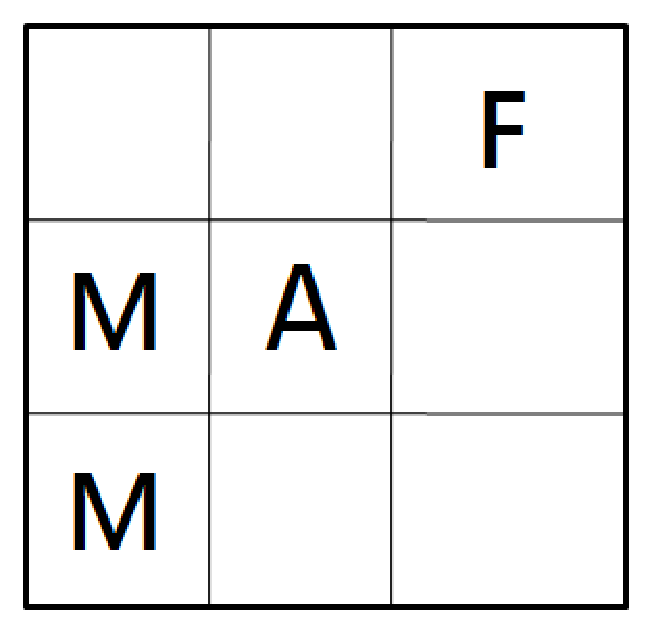
\includegraphics[width=\textwidth] {./figures/monster.eps}
        \caption{A grid world with two monsters (M). A food (F) and an agent (A).}
    \label{fig:Monster}
    \end{minipage}
\end{figure}

Consider the avoid-monster-and-eat-food problem in 
Fig. \ref{fig:Monster}. The world consists of a single agent, a food and a monster.
A reasonable predicate can be $P = {\bf Dist}(O_1, O_2, D)$, which characterizes the
distance between object $O_1$ and $O_2$. The set of literals $I_{P}(S)$ of Fig. \ref{fig:Monster}
is $\{Dist(A, M, 1), Dist(A, M, \sqrt{2}), Dist(A, F, \sqrt{2})\}$.
The domain of constants $\mathbb{D}$ is $\{A, M, F,$ set of some positive real numbers$\}$.
The agent can move in the four possible directions, therefore the action for the agent $\mathbb{A}$ 
is \{North, South, East, West\}.


Though there are many batch learning algorithms available for linear regression, they are not suitable for reinforcement learning
tasks. The batch learning requires a full pass through the data, which not only increases the time
to update the value function as the number of data goes up, but also increases the memory storage. Because 
the value for each time step needs to be stored for the full pass through, it will eventually
exhaust all available memory resources. Thus, online learning is a more appropriate choice
for reinforcement learning. 

There are several Least-Squares Temporal Difference (LSTD) algorithms (\cite{OldLSTD}, \cite{LSTD}, \cite{LSPI} and \cite{TDFA09}) which are proposed for 
learning the value function by basis function approximation for non-relational MDP problems. 
These algorithms conduct linear regression in an online fashion, however, they are not suitable for our 
relational setting. Because we don't have prior knowledge about which relation is relevant to the value function, 
we need to provide a bunch of relations which may be large compared to the samples, and these methods are prone
to over-fitting. 

A approach to avoid over-fitting is to include regularization term in the regression setting. 
Several algorithms for L1 and L2 regularization for TD learning have been proposed (\cite{L1LSTD} and \cite{LassoTD}).
The L1 regularization is particularly suited for our relational setting, since it provide sparse solutions
and can be used as a method for relational template selection.

In this work, we use the approach proposed by Carbonetto et al. \cite{OnlineL1} to estimate the value function.

By estimating the value function by L1-regularized linear regression, we obtain the following relational SARSA algorithm:
\begin{center}
\begin{tabular}{@{}lp{6cm}@{}}
\hline
Algorithm: relational SARSA\\
\hline
Initialize $\hat{Q_0}$ arbitrarily\\
$t \leftarrow 0$\\
Repeat (for each episode)\\
\ \ \ \ \ \ Initialize $s$\\
\ \ \ \ \ \ Choose $a$ based on $s$ using policy derived from $\hat{Q_t}$ (e.g., $\epsilon$-greedy method)\\
\ \ \ \ \ \ Repeat (for each step of episode):\\
\ \ \ \ \ \ \ \ \ \ \ \ Take action $a$, obtain reward $r$ and next state $s'$ from the environment\\
\ \ \ \ \ \ \ \ \ \ \ \ Choose $a'$ based on $s'$ using policy derived from $\hat{Q_t}$ (e.g., $\epsilon$-greedy method)\\
\ \ \ \ \ \ \ \ \ \ \ \ $\hat{q_t} \leftarrow \hat{Q_t}(s, a) + \alpha [r + \gamma \hat{Q_t}(s', a')-\hat{Q_t}(s, a)]$ \\
\ \ \ \ \ \ \ \ \ \ \ \ Update $\hat{Q_t}$ with $(s, a, \hat{q_t})$ by online L1 regression to produce $\hat{Q_{t+1}}$\\
\ \ \ \ \ \ \ \ \ \ \ \ $s \leftarrow s'$\\
\ \ \ \ \ \ \ \ \ \ \ \ $a \leftarrow a'$\\
\ \ \ \ \ \ \ \ \ \ \ \ $t \leftarrow t+1$\\
\ \ \ \ \ \ Until $s$ is terminal\\
\hline  
\end{tabular}
\end{center}




\section{Progressive Transfer Learning}
To speedup the learning process, it is known \cite{KeepAway} that it is beneficial to allow
the agent to learn from simple scenarios first. In this work, we propose a progressive transfer learning 
approach to gradually transfer the knowledge from simple scenarios to a more complex one.

We start from a simple world which contains one object, and learn the utility associated 
with the predicates with only one object involved. Then we gradually increase the number of 
objects involved in each scenario to train the higher order predicates. 

We denote $V^i$ as the Q-function with the state involved $i$ objects. The objective is to
compute $\Delta{V^i(S)} = V^i(S) - V^{i-1}(S)$. Again, we use the linear approximation to estimate $\Delta{V^i}$:
%TODO: show the state in V^i-1 is obtained by ignoring one object of the state
\begin{equation}
\Delta{V^i}(S) = \sum_{L^i_j \in S} V_{L^i_j},
\label{eq:deltaV}
\end{equation}
where $L^i$ is the $i$th-order predicate. $\Delta{V^i}$ indicates the amount of knowledge we need to 
transfer from a simpler model. It is the residual between the current model and the transferred one.
The objective is to learn the residual function for each training process. If the residual function is 
0 everywhere, we achieve the optimal knowledge transfer.
$V_{L^i}$ is the utility associated with the $i$th-order predicate. We can
see that the utility of a higher order predicate is to estimate what cannot be explained by
lower order predicates. 

The value function $V^i$ can be constructed by:
\begin{equation}
    V^i(S) = V^1(S)+\Delta{V^2(S)}+\dots+\Delta{V^i(S)}
\label{eq:deltaSum}
\end{equation}

Combined with the equation \ref{eq:deltaV}, we can get:
\begin{equation}
    V^i(S) = \sum_{L^1_j \in S} V_{L^1_j}+\sum_{L^2_j \in S} V_{L^2_j}+\dots+\sum_{L^i_j \in S} V_{L^i_j},
\label{eq:deltaSum}
\end{equation}
which is corresponding to our original equation \ref{eq:relV}.

%TODO: our hope is that residual decrease as the order goes up
%if so, we don't need to transfer all the way up. We can just use 2vs 1 to go 10vs9 since the approximation is good enough

%Notice that our objective is to learn the utility associated with each relation.

\section{Experiment}


%TODO: the template in this experiment
%TODO: show the difference of the regressed V and the optimal V for a scenario. It indicates our method
% can estimate the unencountered scenario without sample through it. (work on non-repeating scenario).
%Show the effectiveness of reward explanation
%Show the effectiveness of template selection
%Biased Estimation (if not regression, and slower (require a lot of sampling)
%state it's impossible to do with non-relational approach
We show the effectiveness of our algorithm on a simple avoid-monster-and-eat-food problem, which has been shown
in Fig. \ref{fig:Monster}. The world consists of a single agent, a food and a monster.
The location of all objects are randomly generated at the beginning of each episode.
The agent moves within 8 by 8 grid.
There are 10\% chances for the agent to move in a random direction.
%The size of the state space is $8 \times 8 \times 3 ^ (64 - 1)$
It gets a reward of 20 when it gets a food and -30 if it is caught by
a monster. A penalty term -0.1 would apply for each step. If the agent tries to walk out of the world, it will
stay put and receive -1 reward. With 30\% probability, the monster moves one step toward the location of the agent.
Otherwise, it stays in the original location. 
Each episode ends when the food is consumed or the agent is caught by a monster. 

\begin{figure}[h]
    \centering
    \begin{minipage}[t]{0.6\linewidth}
        \centering
        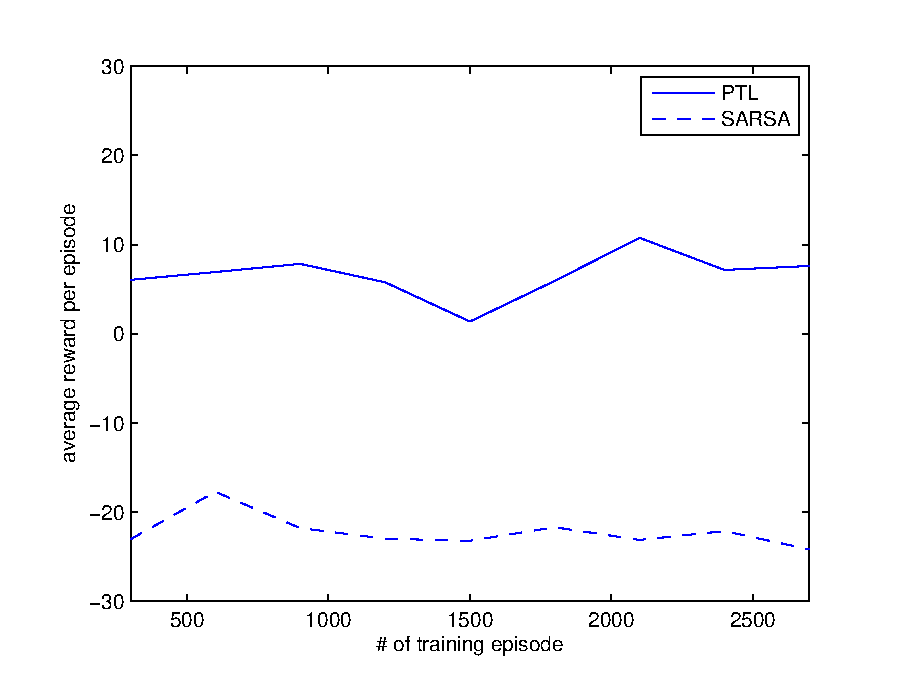
\includegraphics[width=\textwidth] {./figures/RRL_result.eps}
        \caption{The average reward with and without progressive transfer learning}
    \label{fig:Res}
    \end{minipage}
\end{figure}

\begin{figure}[h]
    \centering
    \begin{minipage}[t]{0.6\linewidth}
        \centering
        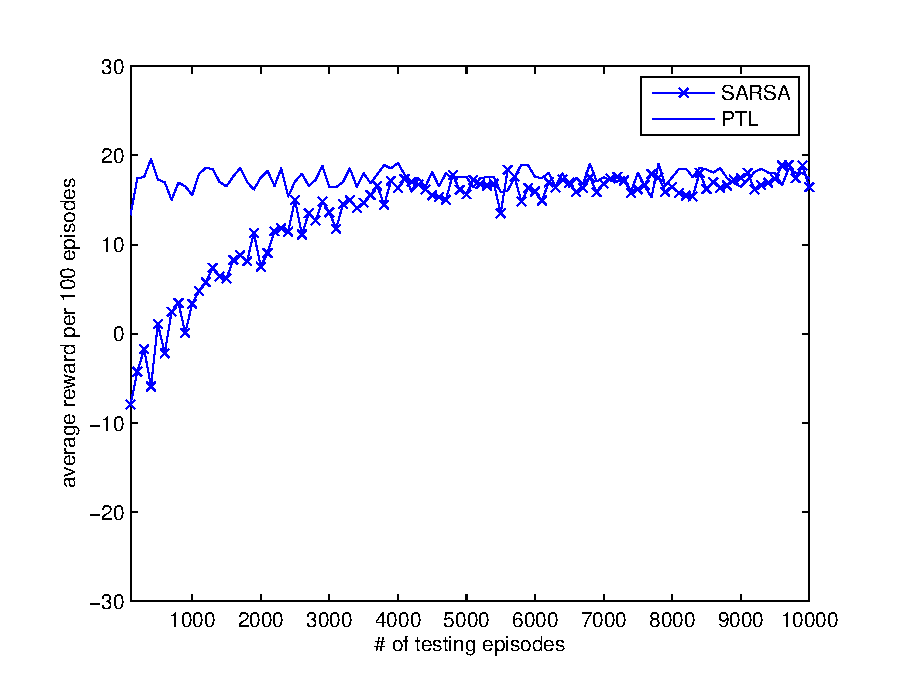
\includegraphics[width=\textwidth] {./figures/Conv.eps}
        \caption{The learning rate of PTL and SARSA agents}
    \label{fig:Res_Learning}
    \end{minipage}
\end{figure}
We compare the result with progressive transfer learning(PTL) and traditional SARSA.
The PTL agent was trained by the simple scenarios with one or two objects. 
The scenario with one object involves the agent itself. The scenarios with two objects involves
the agent and a food or a monster. Each scenario takes one-third of total episodes to train
the agent. The agent needs to transfer its knowledge
from the simple configurations to a more complex testing environment which consists of
three objects with one for each type. The SARSA agent uses all episodes to learn from the complete world, which consists
of three types of objects and is the same as the testing environment. 
Fig. \ref{fig:Res} shows the average reward for 100 episodes. Each agent was trained separately with different number of episodes. 
The figure indicates how the amount of training in the simple scenarios affects the performance of the agent.

Fig. \ref{fig:Res_Learning} shows the learning rate of the PTL and SARSA agents. We trained the PTL agent by 450 episodes.
Then we tested them for 10,000 episodes and average the reward for each 100 episodes. To decrease the time for convergence,
the size of the world is set to 4 by 4 grid and the monster is static.

\begin{figure}[h]
    \centering
    \begin{minipage}[t]{0.6\linewidth}
        \centering
        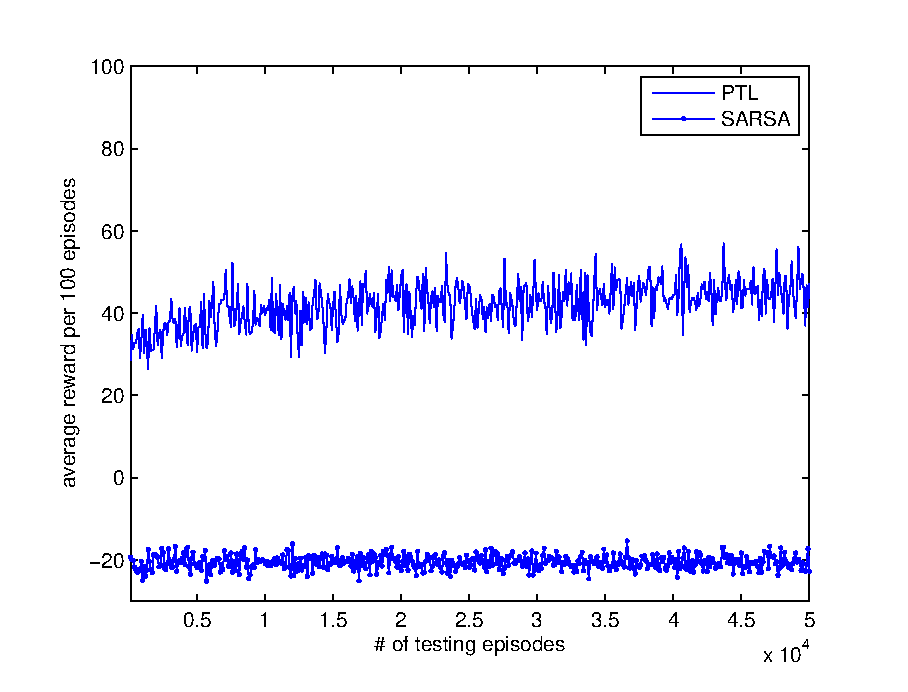
\includegraphics[width=\textwidth] {./figures/Comp.eps}
        \caption{The average reward for the world consists of 5 food and 2 monsters}
    \label{fig:Res_Complex}
    \end{minipage}
\end{figure}

To show that the efficiency for PTL agent to learn in more complex scenario, we tested the agents in a world with
5 food and 2 monsters. The monster moved toward the location of the agent with 30\% probability. The world is 8 by 8. 
The PTL agent was trained for 600 episodes. We run the experiment with 50,000 episodes.
The result is shown in Fig. \ref{fig:Res_Complex}. 



%The size of the state space is more than $3^{64}$, which is impractical to solve with non-factorized and 
%non-relational approach. We compare our approach with the work in \cite{RRLTD}. We first generated 
%1000 episodes and run the experiments with the episodes to ensure the fair comparison.
%The predicates used in the experiment are listed in the table \ref{tbl:Predicates}.

%The result is not generated yet.

%\begin{table}
%\begin{tabular}[h]{ll}
%\hline
%Features used for the predicate construction\\
%\hline
%$locX(O)$&: the x-coordinate of the object $O$\\
%$locY(O)$&: the y-coordinate of the object $O$\\
%$dispX(O_1, O_2)$&: $locX(O_1) - locX(O_2)$\\
%$dispY(O_1, O_2)$&: $locY(O_1) - locY(O_2)$\\
%$class(O)$&: the class of the object $O$\\
%\hline
%\end{tabular}
%\caption{The features used by predicates.}
%\end{table}

%\begin{table}
%\begin{tabular}[h]{ll}
%\hline
%Predicates used in the experiment\\
%\hline
%$P_{locX}(O, X)$&: true when $locX(O) = X$\\
%$P_{locY}(O, Y)$&: true when $locY(O) = Y$\\
%$P_{dispX}(O_1, O_2, \Delta X)$&: true when $dispX(O_1, O_2) = \Delta X$\\
%$P_{dispY}(O_1, O_2, \Delta Y)$&: true when $dispY(O_1, O_2) = \Delta Y$\\
%$P_{template1}(C_1, C_2, O_1, O_2, \Delta X_2, \Delta Y_2)$&: true when $class(O_1) = C_1$\\
                                                           %&\  and $class(O_2) = C_2$ \\
                                                           %&\  and $P_{dispX}(O_1, O_2, \Delta X_2)$\\
                                                           %&\  and $P_{dispY}(O_1, O_2, \Delta Y_2)$\\
%$P_{template2}(C_1, C_2, C_3, O_1, O_2, \Delta X_2, \Delta Y_2, O_3, \Delta X_3, \Delta Y_3)$&: true when \\
                                                                                             %&\ $P_{template1}(C_1, C_2, O_1, O_2, \Delta X_2, \Delta Y_2)$ \\
                                                                                             %&\ and $P_{template1}(C_1, C_3, O_1, O_3, \Delta X_3, \Delta Y_3)$ \\
%$P_{templateN}(C_1, \dots, C_N, O_1, O_2, \Delta X_2, \Delta Y_2, \dots, O_N, \Delta X_N, \Delta Y_N)$&: true when\\
                                                                                             %&\ $P_{template1}(C_1, C_2, O_1, O_2, \Delta X_2, \Delta Y_2)$ \\
                                                                                             %&\ \ \ \ \ \ \vdots \\
                                                                                             %&\ and $P_{template1}(C_1, C_N, O_1, O_N, \Delta X_N, \Delta Y_N)$ \\
%\hline
%\end{tabular}
%\caption{The predicates for grid world games.}
%\label{tbl:Predicates}
%\end{table}

%We conduct our experiment in $8 \times 8$ grid world. 
%The world consists of an agent, indefinite number of coins and monsters. 
%The location and the number of coins and monsters are decided at the beginning of each episode.
%The goal of the agent is to collect as much coins as possible. Each coin contributes $+10$ reward to the agent.
%After all coins have been collected, the episode ends. If the agent encounters a monster, it will receive
%$-30$ reward and the episode ends immediately. The agent will receive $-1$ reward for each step. 

%Unlike the grid world in previous literature, this game is more challenging because
%the agent faces different scenarios for each episode. It is unlikely that
%an episode will ever repeat itself. The success of the agent lies in how
%to learn from the previous episode and transfer it into the new one.

%The discounted reward factor $\gamma$ is 0.9 and $\alpha$ is 0.2.
%The exploration strategy is $\epsilon-greedy$ with $\epsilon$ equal to 0.2.
%Fig. \ref{fig:AvgReward} shows the average reward per step for the agent.
%Fig. \ref{fig:Policy} shows the learned policy of individual object class after 2,000,000 steps.
%%It indicates that 

%Figure 1: Our agent (S) roams an n by n grid. It gets a payoff of 0.5 for every
%time step it avoids predator (P), and earns a payoff of 1.0 for every piece of food
%(f) it finds. S moves two steps for every step P makes, and P always moves directly
%toward S. When food is found, it reappears at a random location on the next time
%step. On every time step, S has a 10% chance of ignoring its policy and making a
%random move.



%hard to define good concepts "concept" -> feature selection, expert is not reliable
%quote by Eric
% Selection the relevent template of the value function
%enable to differenciate the source of rewards -> regression, they heuristicly sum them up to get the value function
%What is relational template? (capture the local property of a problem and ignore the rest)
%hich applies 
% no prior knowledge about transition and rewards
%model free approach

%TODO: vision perspective-->How to use policy to recognize objects.
%TODO: strength: I found a way to decompose the value function of factoerized MDP into sum of local functions of primitive predicates
% I can change it to sum of composite predicate as well like Relational Temporal Difference Learning by Nima


\section{Rate of Convergence}
Let $V^N = V(O_1, \dots, O_N)$ be the value function of a game which consists of $N$ objects of the same type.
Each object has $K$ states. Therefore, the number of states for $N$ object world is $K^N$.
Our objective is to approximate $V^N$ by:
\begin{equation}
    \hat{V}^N(O_1, \dots, O_N) = \sum_{1 \le i_1 \le N} \Delta V^1(O_{i_1}) + \sum_{1 \le i_1, i_2 \le N} \Delta V^2(O_{i_1}, O_{i_2})
    + \dots + \sum_{1 \le i_1, \dots, i_{N-1} \le N} \Delta V^{N-1}(O_{i_1}, \dots, O_{i_{N-1}})
\end{equation}

\begin{theorem}
Let $R = \max_x |\Delta V^1(x)|$, the magnitude of the largest expected reward in the one object world.
If there exists a constant $a$, $0 < a < 1$, such that $a^iR > \max_x |\Delta V^{i+1}(x)|$ for all $i>1$,
we can achieve $\epsilon$-optimality ($|V^N - \hat{V}^N| < \epsilon$) within total steps $O(MK^{2i^*})$.
\end{theorem}

Proof:\\
Assume we know the transition probability, therefore we can use dynamic programming to solve the MDP problem.
Following the analysis of value iteration in \cite{ComplexityMDP}, we can solve $\Delta V^1 \equiv V^1$ in 
$O(MK^2)$ steps, where $M$ is the number of possible actions. Likewise, $\Delta V^i \equiv V^i - V^{i-1}$ can be computed in $O(MK^{2i})$ steps.
To achieve $\epsilon$-optimality ($|V^N - \hat{V}^N| < \epsilon$), we need to compute the value function up to $i^*$ order, where 
$i^* > \frac{log(\epsilon) - log(R)}{log(a)}$. As a result, the total steps are $O(MK^2) + O(MK^{4}) + \dots + O(MK^{2i^*}) = O(MK^{2i^*})$.
Compared to use dynamic programming to solve the problem directly, it requires $O(MK^{2N})$ steps. When $N \gg i^*$, it is a significant performance boost.

The above analysis assumes the magnitude of the value function decreases a constant factor as the order goes up.
Let's change to a different assumption.

\begin{theorem}
If there are at most $L$ nonzero values for $\Delta V^i$, $i > 1$, we can learn the value 
function with $O(ML^2)$ steps.
\end{theorem}

Proof:\\
To learn $\Delta V^1$ still requires $O(MK^2)$ step. However, $\Delta V^2$ has only $L$ nonzero values. We
can run dynamic programming algorithm specifically to the nonzero locations, which requires $O(ML^2)$.
The overall steps are $O(MK^2) + O(NML^{2})$. When $K^N \gg L$, it can be a huge performance boost as well.

\begin{figure}[h]
    \centering
    \begin{minipage}[t]{0.6\linewidth}
        \centering
        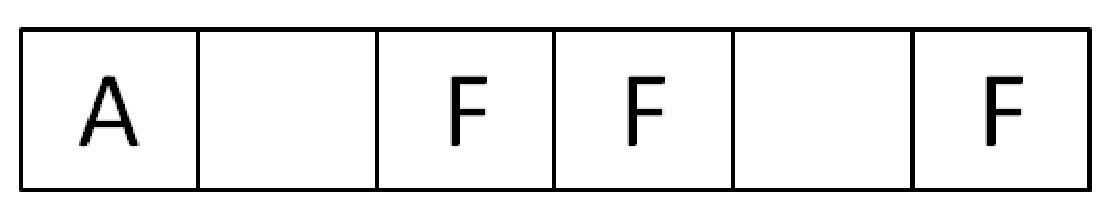
\includegraphics[width=\textwidth] {./figures/EasyExample.eps}
        \caption{A game whose value function can be approximated by first order templates }
    \label{fig:EasyGame}
    \end{minipage}
\end{figure}

Fig. \ref{fig:EasyGame} illustrates a game which satisfies with the assumption of both of the above theorems. 
The agent always starts 
from the leftmost of the grids. The agent receive reward $R$ when it gets a food. The only action of the agent is to go to the right. The discount factor
is $\gamma$. Suppose the food are $F=\{F_1, F_2, \dots, F_N\}$. The value function of a food and an agent
is $\Delta V^1(F_k, A) = \gamma^{d_k}R$, where $d_k$ is the distance between the food and the agent.
The value function for this game is simply $V(F, A)=\sum_k \Delta V^1(F_k, A)$.
The value function of higher order templates are all zeros ($\Delta V^2=\Delta V^3=\dots=\Delta V^N=0$).
Therefore, we can always find a constant $a$ to satisfy $a^iR > \max_x |\Delta V^{i+1}(x)| = 0$ for all $i>1$. 


\begin{figure}[h]
    \centering
    \begin{minipage}[t]{0.6\linewidth}
        \centering
        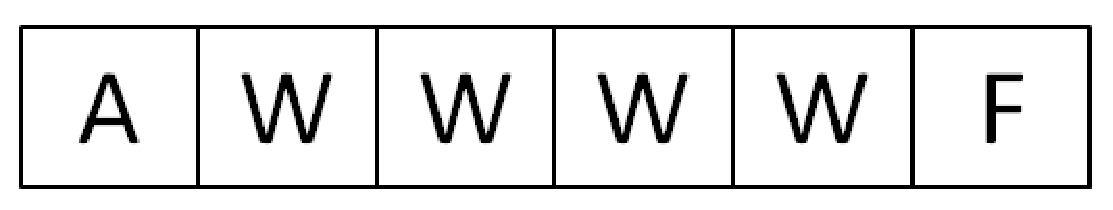
\includegraphics[width=\textwidth] {./figures/WallExample.eps}
        \caption{A game whose value function cannot be approximated well by lower order templates}
    \label{fig:WallExample}
    \end{minipage}
\end{figure}
Fig. \ref{fig:WallExample} shows a similar game which includes additional "wall" objects.
This game serves as an example to show when the preconditions of the above theorems cannot be satisfied.
The game consists of an agent, a food and several wall objects. The agent always starts
from the leftmost of the grids, while the food always appear at the rightmost of the grids.
There are several walls between them. The wall blocks the path of the agent, so the agent
cannot get the food after the wall. Assume discount factor for this game is 1.
Let the walls be $W = \{W_1, W_2, \dots, W_N\}$.
$\Delta V^1(F, A) = 1^{d_k}R = R$. Since the agent cannot get any reward from walls, $\Delta V^1(W_k, A) = 0$
However, $V(F, W_k, A) = 0 = \Delta V^1(F, A) + \Delta V^1(W_k, A) + \Delta V^2(F, W_k, A) = R + 0 + \Delta V^2(F, W_k, A)$.
As a result, $\Delta V^2(F, W_k, A) = -R $. Similarly, $V(F, W_k, W_j, A) = 0 = \Delta V^1(F, A) + \Delta V^1(W_k, A) + \Delta V^1(W_j, A) + \Delta V^2(F, W_k, A) + \Delta V^2(F, W_j, A) + \Delta V^3(F, W_k, W_j, A)
= R + 0 + 0 -R -R + \Delta V^3(F, W_k, W_j, A)$. We get $\Delta V^3(F, W_k, W_j, A)=R$. Repeat this process, we get $|V^N(F, W, A)| = R$ for any $N>0$.
It is impossible to find the constant $a$ for this game.

If we let the discount factor to be less than 1, we get $|V^N(F, W, A)| \le \gamma^{N+1}R$. 
It satisfy the conditions of the theorem 1 but does not satisfy conditions of theorem 2.

\begin{figure}[h]
    \centering
    \begin{minipage}[t]{0.6\linewidth}
        \centering
        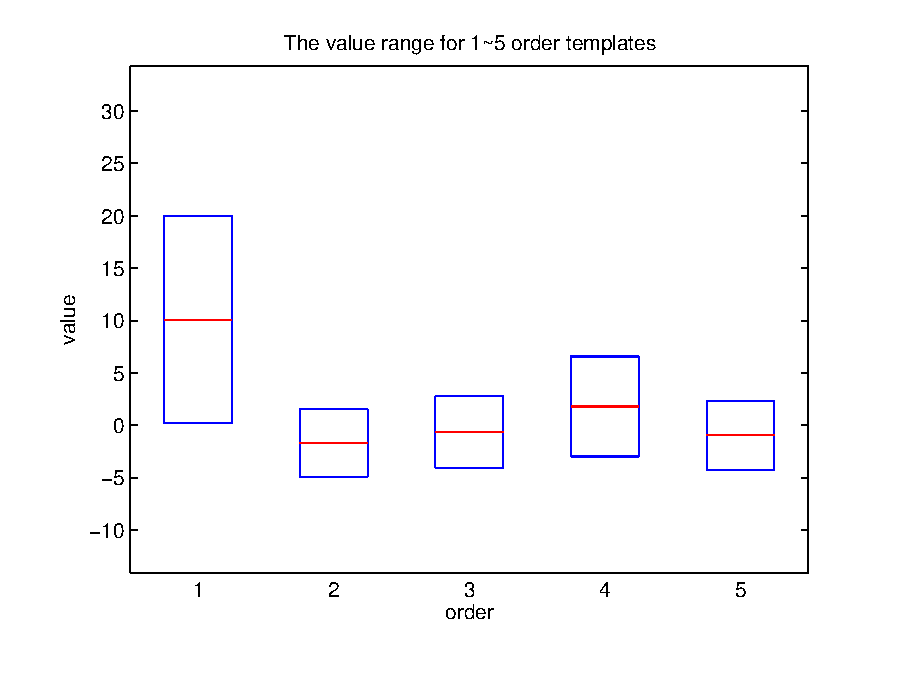
\includegraphics[width=\textwidth] {./figures/ValueOfOrder.eps}
        \caption{The value range for the first five order templates}
    \label{fig:ValueOrder}
    \end{minipage}
\end{figure}

To evaluate if the magnitude of value function would diminish as the order increases, 
we run the game which is similar to Fig. \ref{fig:EasyGame}, but the agent can be placed to anywhere,
and it can choose to move to left or right.
The result is shown in Fig. \ref{fig:ValueOrder}. It indicates that the magnitude of value drops from 
first order to second order, however, we do not observe the trend continues. 
This example that does not satisfy either of theorem 1 or 2, but it still shows speedup
in our experiment.
Clearly the conditions of theorem 1 and 2 are sufficient but not necessary for the 
speedup of transfer learning.

\begin{figure}[h]
    \centering
    \begin{minipage}[t]{0.6\linewidth}
        \centering
        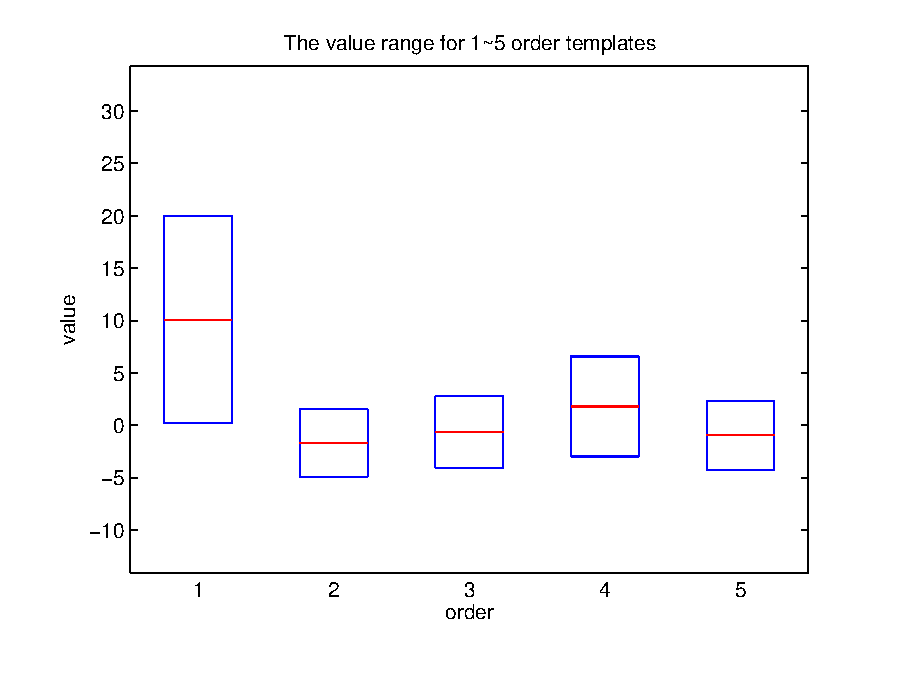
\includegraphics[width=\textwidth] {./figures/ValueOfOrder.eps}
        \caption{The value range for the first five order templates}
    \label{fig:ValueOrder}
    \end{minipage}
\end{figure}


\begin{figure}[h]
    \centering
    \begin{minipage}[t]{1.0\linewidth}
        \centering
        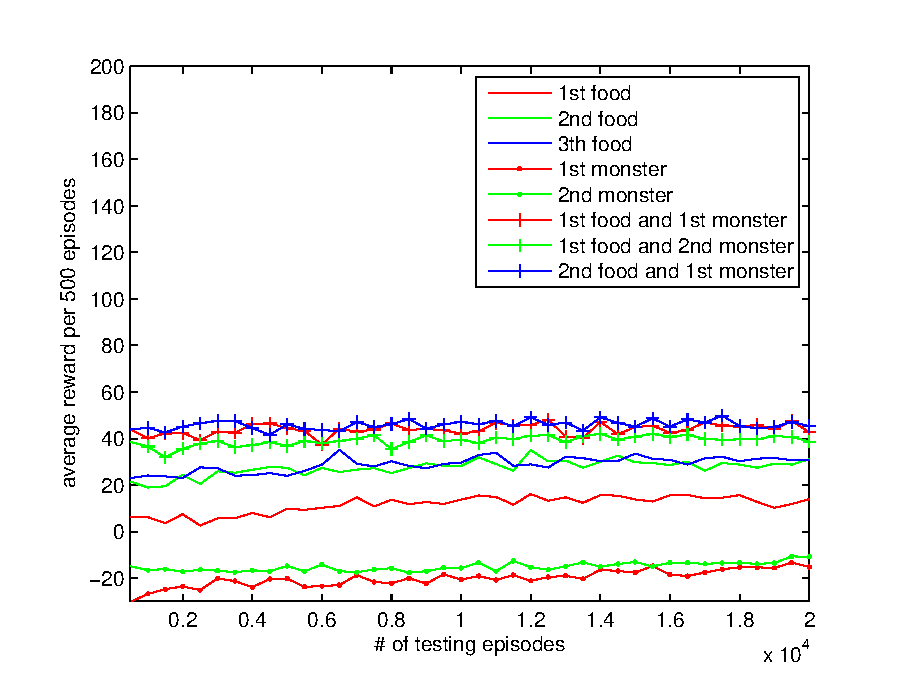
\includegraphics[width=\textwidth] {./figures/TemplateOrder.eps}
        \caption{The comparison of the effectiveness of different order of templates}
    \label{fig:TemplateOrder}
    \end{minipage}
\end{figure}

To show the effectiveness of higher order templates, we run the game with 5 food and 2 monsters
and compare the average reward of them. The result is shown in Fig. \ref{fig:TemplateOrder}.
Each agent has 10,000 training episodes which are evenly distributed among different templates.
Then we run it for additional 20,000 episodes to test. It indicates that under the 
same amount of training, the agents which are trained in complex environments perform 
better than those without. However, the benefits diminish after a certain order.
For example, the agent trained with 2 food performs better than the agent trained with 1 food.
But the agent trained with 3 food performs almost the same as the 2 food one.
In addition, the higher order may not be always better than lower order.
The agent which is trained with 1 food and 2 monster does not perform better than 
1 food and 1 monster. It maybe due to the fact that it's harder for the agent to learn
in 2 monster environment.

\section{Related Work}
The relational reinforcement learning is one of the recent research direction for RL community. 
We provide brief review here. More complete review can be found in \cite{TadSurveyRRL} and \cite{OtterSurveyRRL}.
The relational representation allows us to generalize the existing policy into the complex world, transfer
the knowledge to similar scenarios and handle problems with varying number of objects.
Driessens et al.\cite{TG} combined the Tilde algorithm and the G-algorithm to construct a
relational regression tree to predict Q values. 
%TODO: the approach discovers a huge regression tree for every scenario, which forbids the knowledge transfer
The instance based regression approach \cite{KNN_RRL} computes the weighted average of Q values from the stored
examples. The weights are determined by the distance between the examples.
G\"{a}rtner et al. \cite{GraphKernel} adopted Gaussian processes to approximate Q-functions. Since
Gaussian processes require positive definite covariance function to work, they regards the relations as graphs and
use graph kernels as the covariance function.

There are several works which decompose the value function into several local functions. 
Russel et al.\cite{RessellDecompose} proposed to build a RL agent from simpler subagents. Each subagent has its own
reward function. The value function is the sum of local functions which are learned by each
subagent individually. Guestrin et al.\cite{RelationalMDP} approximates the value function by
linear combination of local functions which are defined for each class of objects.

%TODO: regularized regression approach here
%The approach by Walker et al. (2004) separates the structural induction of the representation
%from the actual value function estimation. First a set of first-order features
%– represented by relational conjunctions over state atoms – is induced. These are then
%used as input for a regression algorithm that estimates Q-value functions per action. The
%method resembles standard function approximation methods for RL (see Section 3.6), using
%first-order features and regularized kernel regression for learning the value function.
%The method resembles standard function approximation methods
%for RL (see Section 2.3.1), using first-order features and regularized kernel regression for
%learning the value function. However, instead of Q-learning, Monte Carlo estimates using
%hand-coded policies are used as training examples.

More recently, Asgharbeygi et al. \cite{RRLTD} proposed relational temporal difference learning 
to learn a distributed value function represented over a conceptual hierarchy of relational predicates. 
Proper et al. \cite{RelationalTemplate} uses relational templates to transfer the knowledge from different 
subdomains of a real-time strategy game. These approaches both approximates the value function by 
the sum of several local functions which are defined over relational predicates or templates. There
are some issues of their approaches. First, they both require an "expert" to define appropriate
predicates or templates. The "expert" may miss some important templates which are necessary for 
the agent to succeed. He may also define some redundant templates so the learning process 
becomes redundant. The second issue is that when an agent receives a reward, they use the reward to update all of the 
local functions. However, the reward may actually be generated by one of the functions, not all of them.
Their approaches are unable to determine the cause of the reward.

In this work, we propose a relational template selection approach to 
select a set of relevant relational templates by L1-regularized regression.
The L1-regularized regression allows us to define a large number of relational
templates and select the relevant templates automatically. Therefore, we do not require
a set of good expert-defined templates. The regression also allows us to explain the cause of the reward.
A reward received by the agent would be explained away by some of the local functions, so it cannot
be claimed by all local functions at the same time.

%Our method resembles standard function approximation methods for RL (Guestrin),
%using first-order features and regression to learn the value function. 
%Nevertheless, in our relational setting, the number of features as well as basis functions are not fixed, but 
%may vary over time.

%Our work is the first who adopts L1 regression on relational reinforcement learning.

%TODO: state the differences with hierarchical approaches

\endinput
%coarse to fine template construction (why it will select coarse template first? because it appears more than complex templates)
%\section{Regression}
%coarse to fine template selection (why it will select coarse template first? because it appears more than complex templates)
%why L1?
%why use online L1?
%how to update the value V by regressed Vhat
%model free
%unknown transition and reward
%find the relevant template


%Another closely related line of work comes from
%Guestrin et al. (2003), who report a system that di-
%rectly approximates the value function by additively
%decomposing it into local functions for each class of
%objects, then calculating weights for the combina-
%tion by solving a linear program using constraint-
%sampling methods. Their approach assumes that re-
%lations among objects do not change over time. Our
%method does not make that assumption, as our learned
%value function is defined over relational predicates
%rather than classes of objects. Less closely related
%Relational Temporal Difference Learning
%approaches include approximate policy iteration (e.g.,
%Fern et al., 2004) and explanation-based reinforcement
%learning (e.g., Boutilier et al., 2001).

%There are many implicit and explicit formalizations of relational versions of MDPs.
%Implicit formalizations (see for example (Guestrin et al., 2003a; Guestrin, 2003; Kersting
%and De Raedt, 2004; Kersting et al., 2004; Fern et al., 2003, 2004; Yoon et al., 2002; Boutilier
%et al., 2001)) use a (fragment of a) first-order language to specify abstract definitions of
%e.g. transition functions and as a consequence, – in an implicit way – an underlying,
%ground relational MDP is specified; i.e. it consists of the semantic level of the language
%used. Explicit formalizations (see for example (Mausam and Weld, 2003; van Otterlo and
%Kersting, 2004; Roncagliolo and Tadepalli, 2004; van Otterlo, 2004)) explicitly define new
%versions of MDPs where the states and actions are defined using ground relational atoms;
%a first-order language is then typically used for abstraction over this MDP definition. Both
%types of formalizations are clearly interchangeable and the main important aspect is the
%relation between the logical abstraction language and the underlying MDP it models. In
%this paper we use a simple definition of an RMDP (van Otterlo, 2004):


%In model-free relational RL, one has studied different
%relational learners for function approximation
%(D·zeroski et al., 2001; Lecoeuche, 2001; Driessens &
%Ramon, 2003; GÄartner et al., 2003). Others have applied
%Q-learning based on pre-speci¯ed abstract state
%spaces: Kersting and De Raedt (2003) investigate pure
%Q-learning, Van Otterlo (2004) learns the Q-function
%via learning the underlying transition model. Fern
%et al. (2003) extended previous work on upgrading
%learned policies for small relational MDPS (RMDPs)
%with approximated policy iteration. Finally, Guestrin
%et al. (2003) recently reported on class-based, approximate
%value functions for RMDPs.

%By contrast, previous work on relational reinforce-
%ment learning has focused on different responses to
%the above challenges. Dzeroski et al. (2001) adapted
%relational regression algorithms to take advantage of
%relational structure in describing Q values. For ex-
%ample, the TG algorithm (Driessens et al., 2001) in-
%duces a relational regression tree that predicts Q val-
%ues. However, our system relies on state values so
%that the learning algorithm makes explicit use of the
%domain description.
%Another closely related line of work comes from
%Guestrin et al. (2003), who report a system that di-
%rectly approximates the value function by additively
%decomposing it into local functions for each class of
%objects, then calculating weights for the combina-
%tion by solving a linear program using constraint-
%sampling methods. Their approach assumes that re-
%lations among objects do not change over time. Our
%method does not make that assumption, as our learned
%value function is defined over relational predicates
%rather than classes of objects. Less closely related
%Relational Temporal Difference Learning
%approaches include approximate policy iteration (e.g.,
%Fern et al., 2004) and explanation-based reinforcement
%learning (e.g., Boutilier et al., 2001).


%Through the use of relational regression������ the RRL sys
%tem 	Dzeroski et al������ 
 %allows the application of
%almost standard Qlearning to reinforcement learning
%problems in environments that are characterized by
%their relational nature
%The use of relational representations of states and
%actions combined with relational regression for Q
%function generalization allows the use of structural in
%formation such as the existence of objects with the
%right properties or relations between objects in the de
%scription of the Qvalues������ and as a consequence in the
%description of the derived policy This enables the re
%use of experience on smaller but related problems when
%confronted with more elaborate or simply larger tasks
%Three regression algorithms have been developed for
%use in this RRL system the TG algorithm������ which in
%crementally builds rst order regression trees������ an in
%stance based algorithm called RIB and a kernel based
%algorithm KBR that uses Gaussian processes as the
%regression technique
%The TG algorithm 	Driessens et al������ 
 %is a combi
%nation of the Tilde algorithm 	Blockeel  De Raedt������
%
 %that builds rst order classication and regres
%sion trees and the Galgorithm 	Chapman  Kael
%bling������ 
 %that uses a number of statistical values
%concerning the performance of each possible extension
%in each leaf of the tree to build the tree incrementally
%The relational regression trees used by the TG algo
%rithm use conjunctions of rst order literals as tests in
%the internal leafs The test corresponding to a certain
%leaf is the conjunction of the tests appearing on the
%path from the root of the tree to the leaf������ in which any
%appearing variable is existentially quantied The TG
%algorithm employs a userdened renement operator
%that originated in the Tilde system to generate the
%possible rst order tests that can be used to replace
%a leaf The statistics stored by the TG algorithm al
%gorithm in each leaf of the tree consist of the number
%of examples classied positively or negatively by each
%possible test and the sum of the Qvalues and squared
%Qvalues in each of these cases This allows the use
%of an Ftest to decide which test to select For now������
%no tree restructuring is done by TG All decisions that
%the algorithm makes are nal
%The instance based algorithm RIB 	Driessens  Ra
%mon������ 
 %uses knearestneighbor prediction as the
%regression technique������ ie������ it computes a weighted av
%erage of the Qvalues of the examples stored in mem
%ory where the weight is inversely proportional to the
%distance between the examples The distance used
%needs to be able to cope with relational representa
%tions of states and actions and can be either a gen
%eral purpose rst order distance 	Sebag������  Ra
%mon  Bruynooghe������ 
 %or an applicationspecic
%one������ which can usually be computed more e
ciently
%Because Qlearning generates a continuous stream of
%learning examples������ a number of example selection
%methods were developed to reduce both the memory
%and the computational requirements These selection
%criteria are based on those used in IB and IB 	Aha
%et al������ 
 %and look at the inuence of individual
%examples on the overall prediction error
%The third algorithm is called KBR 	Gartner et al������
%a
 %and uses Gaussian processes as the regression
%technique Gaussian processes 	MacKay������ 
 %require
%a positive denite covariance function to be dened
%between the example descriptions Because of the use
%of relational representations in the RRL system������ ker
%nels for structured data have to be used to fulll this
%task Possible candidates here are the convolution
%kernel 	Haussler������ 
 %or kernels dened on graphs
    %Gartner et al������ b
% Because Gaussian processes
%are a Bayesian technique������ the KBR algorithm oers
%more than just a basic prediction of the Qvalue of a
%new unseen example It can also give an indication of
%the expected accuracy of this estimate������ which in turn
%can be used������ for example������ by the Qlearning algorithm
%to guide exploration
%One of the major problems that reduces the applica
%bility of Qlearning with relational function abstrac
%tion stems from the nature of Qvalues themselves������ ie������
%their implicit encoding of both the distance to and the
%size of the next reward These can be very hard to
%predict in stochastic and highly chaotic tasks Other
%approaches such as advantage learning or policy itera
%tion seem more appropriate in such cases

%update by Q by local value function or the global one? (which one will converge faster?)
%context independent ??

%Weakness of current approach
%TG uses a big classification tree to learn all policy of the agent in its lifetime, we need a new way to find the policy against local structure, for transfer
%

%Handle dynamic number of objects (what if a class is missing?) what is the regression tree work?
%Learn simple scenario from complex one--
%Peter Stone's soccer need a simple scenario to transfer
%But in video games we cannot do it
%Current approach cannot transfer from complex one to simple one, how can it be done? From two block to three blocks
%Hanlde real value relations
%Implement the current approach
%the system dynamics and rewards

%spatial proximity
%temporal proximity
%structure learning, group small number of objects into bigger one (CVPR 2010, Yu Pen Fei's project)



at the level of a template for a task domain. Given a particular
environment within that domain, it defines a specific MDP
instantiated for that environment. The domain is specified by a schema,
which specifies a set of object classes C = fC1; : : : ;Ccg. Each class
C is also associated with a set of state variables S[C] =
fC:S1; : : : ;C:Skg, which describe the state of an object in
that class. Each state variable C:S has a domain of possible
values Dom[C:S]. We define SC to be the set of possible
states for an object in C, i.e., the possible assignments to the
state variables of C.
For example, our Freecraft domain might
have classes such as Peasant, Footman, Gold;
the class Peasant may have a state variable
Task whose domain is Dom[Peasant:Task] =
fWaiting, Mining, Harvesting, Buildingg, and a state
variable Health whose domain has three values. In this
case, SPeasant would have 4  3 = 12 values, one for each
combination of values for Task and Health.
The schema also specifies a set of links L[C] =
fL1; : : : ;Llg for each class representing links between objects
in the domain. Each link C:L has a range [C:L] = C0.
For example, Peasant objects might be linked to Barrack
objects — [Peasant:BuildTarget] = Barrack, and to the
global Gold and Wood resource objects. In a more complex
situation, a link may relate C to many instances of a
class C0, which we denote by [C:L] = fC0g, for example,
[Enemy:My Footmen] = fFootmang indicates that an instance
of the enemy class may be related to many footman instances.
A particular instance of the schema is defined via a
world !, specifying the set of objects of each class; we use
O[!][C] to denote the objects in class C, and O[!] to denote
the total set of objects in !. The world ! also specifies
the links between objects, which we take to be fixed
throughout time. Thus, for each link C:L, and for each
o 2 O[!][C], ! specifies a set of objects o0 2 [C:L], denoted
o:L. For example, in a world containing 2 peasants,
we would have O[!][Peasant] = fPeasant1;Peasant2g;
if Peasant1 is building a barracks, we would have that
Peasant1:BuildTarget = Barrack1.
The dynamics and rewards of an RMDP are also defined
at the schema level. For each class, the schema
specifies an action C:A, which can take on one of several
values Dom[C:A]. For example, Dom[Peasant:A] =
fWait, Mine, Harvest, Buildg. Each class C is also associated
with a transition model PC, which specifies the probability
distribution over the next state of an object o in class
C, given the current state of o, the action taken on o, and the
states and actions of all of the objects linked to o:
PC(S0
C j SC;C:A;SC:L1 ;C:L1:A; : : : ;SC:Ll ;C:Ll:A): (1)
For example, the status of a barrack, Barrack:Status0,
depends on its status in the previous time step, on
the task performed by any peasant that could build it
(Barrack:BuiltBy:Task), on the amount of wood and gold, etc.
The transition model is conditioned on the state of C:Li,
which is, in general, an entire set of objects (e.g., the set of
peasants linked to a barrack). Thus we must now provide
a compact specification of the transition model that can depend
on the state of an unbounded number of variables. We
can deal with this issue using the idea of aggregation [10].
In Freecraft, our model uses the count aggregator ], where
the probability that Barrack:Status transitions from Unbuilt to
Built depends on ][Barrack:BuiltBy:Task = Built], the number
of peasants in Barrack:BuiltBy whose Task is Build.
Finally, we also define rewards at the class level. We assume
for simplicity that rewards are associated only with the
states of individual objects; adding more global dependencies
is possible, but complicates planning significantly. We define
a reward function RC(SC;C:A), which represents the contribution
to the reward of any object in C. For example, we
may have a reward function associated with the Enemy class,
which specifies a reward of 10 if the state of an enemy object
is Dead: REnemy(Enemy:State = Dead) = 10. We assume
that the reward for each object is bounded by Rmax.
Given a world, the RMDP uniquely defines a ground factored
MDP !, whose transition model is specified (as usual)
as a dynamic Bayesian network (DBN) [3]. The random variables
in this factored MDP are the state variables of the individual
objects o:S, for each o 2 O[!][C] and for each
S 2 S[C]. Thus, the state s of the system at a given point in
time is a vector defining the states of the individual objects in
the world. For any subset of variablesX in the model, we define
s[X] to be the part of the instantiation s that corresponds
to the variables X. The ground DBN for the transition dynamics
specifies the dependence of the variables at time t+1
on the variables at time t. The parents of a variable o:S are
the state variables of the objects o0 that are linked to o. In our
example with the two peasants, we might have the random
variables Peasant1:Task, Peasant2:Task, Barrack1:Status,
etc. The parents of the time t + 1 variable Barrack1:Status0
are the time t variables Barrack1:Status0, Peasant1:Task,
Peasant2:Task, Gold1:Amount andWood1:Amount.
The transition model is the same for all instances in the
same class, as in (1). Thus, all of the o:Status variables for
Figure 2: Freecraft tactical domain: (a) Schema; (b) Resulting factored
MDP for a world with 2 footmen and 2 enemies.
barrack objects o share the same conditional probability distribution.
Note, however, that each specific barrack depends
on the particular peasants linked to it. Thus, the actual parents
in the DBN of the status variables for two different barrack
objects can be different.
The reward function is simply the sum of the reward functions
for the individual objects:
R(s; a) = X
C2C
X
o2O[!][C]
R(s[So]; a[o:A]):
Thus, for reward function for the Enemy class described
above, our overall reward function in a given state will be
10 times the number of dead enemies in that state.
It remains to specify the actions in the ground MDP. The
RMDP specifies a set of possible actions for every object in
the world. In a setting where only a single action can be taken
at any time step, the agent must choose both an object to
act on, and which action to perform on that object. Here,
the set of actions in the ground MDP is simply the union
[o2!Dom[o:A]. In a setting where multiple actions can be
performed in parallel (say, in a multiagent setting), it might
be possible to perform an action on every object in the domain
at every step. Here, the set of actions in the ground MDP is a
vector specifying an action for every object: o2!Dom[o:A].
Intermediate cases, allowing degrees of parallelism, are also
possible. For simplicity of presentation, we focus on the multiagent
case, such as Freecraft, where, an action is an assignment
to the action of every unit.
Example 2.1 (Freecraft tactical
Any text after an \endinput is ignored.
You could put scraps here or things in progress.

Objective: Allow computer to play video games
Objective2: perfect modeling
abundance of old games
home robot entertaunnent(kinetics) join the family
Approach:
Input: Screen and Reward function
1. Video Analysis 
2. Control the game by RL algorithms--RL algorithms must be able to be applied to different games successfully
3. Modeling dynamics(the agent needs to explore the game to get enough information)

Comparison to previous work:
1. Nonintrusive gaming(compared to NIPS 2008)
2. Modeling the game
Chanllenge:
1. Real-Time Video Anaylysis
2. A generic RL algorithm which works on different games
Unlike previous work on RL, the objective is not to design a good AI for a specific game to against
human player, the objective is to design a good and generic AI for play different games successfully
But it is not required to be perfect or optimal. AI in video games cannot be perfect, otherwise it 
would be not possible for a human player to beat the game. The opponent is suboptimal in nature.
3. Little prior knowledge on the games. Unlike keep away, it's not possible to design heiracial action
for (Pong). It must be able to play the game from primitive actions or construct the complex actions by itself.
Volleyball
Example: 
  Fireball vs Soccer ball
  In one game, it's necesart to intercept the soccer ball.
  In another game, it's lethal to touch any ball.
4. Huge game states(640X480X30X(256) per seconds), highly redudunet
5. Little training time (the game has 30fps), cant increase that
6. Dynamic number of agents(avoid ball)(different from soccer)(the number of player is dynamics (unlike game theory))

Motivation for reinforcement learning

Articial Intelligence algorithms that can play classic or video games have been studied ex-
tensively. Research in classic games has resulted in Deep Thought for chess [Campbell et al., 2002],
Chinook for checkers [Schaeer et al., 2005], TD-Gammon for backgammon [Tesauro, 1994],
and Polaris for poker [Bowling et al., 2009]. For AI researchers who work on solving vari-
ous games, there is a recurring question that needs to be addressed: why dedicate limited
resources to solving games instead of tackling the real-world problems in which the eld of
Articial Intelligence can contribute to the daily quality of human lives? In other words,
why spend resources on solving chess, if what we need is self-driving cars with near zero
collision rates? Why play checkers, if what we want is an intelligent maid robot that can
cook, vacuum, and wash the dishes?
The motivation for developing AI agents that can play games is threefold. First, games
oer controlled, well-understood, and easily abstracted environments, with well-dened mea-
sures of success and failure. These properties make games suitable platforms for developing
and testing AI algorithms. The methods developed and the knowledge gained from work-
ing in these controlled environments can later be applied to the real-world problems which
are generally messier and harder to measure performances, but still require the same AI
sophistication.
Additionally, games are excellent platforms for showcasing the capabilities of the latest
AI techniques to the public. In 1997, when Deep Blue defeated Garry Kasparov, a great
wave of excitement was generated among regular, non-academic people about Articial
Intelligence. This is because people understand chess, and respect the complexity involved
in playing it well. Back in 1997, the AI community was not able to develop collision-free
autonomous cars or achieve many other longer-term goals of the eld. Showcasing an agent
that mastered chess helped the public understand what the AI community was capable of
at the time.
Finally, with the recent growth of commercial video games into a multibillion-dollar
industry, there is now even more motivation for studying agents that can learn to act intelli-
gently in games [Lucas, 2009, Laird and Lent, 2000]. Non-repetitive, adaptive, interesting,
and in summary intelligent behavior oers a competitive edge for commercial games. As
the game graphics peak at image-like quality, and as the game consoles oer more and more
computational power that can be spent on complex learning algorithms, the importance of
3


Application:
1. desktop (sort the data row??)
2. gaming ( a alternative of in game AI) can act as opponent or friends (human and computer cooperation)( with 2 different computers)
3. game modeling ( convert to another platform)
2. simulatioin env forj robot
4. agent in online gaming (need to go to toilet)
5. General in game AI
6. General in computer sceice (viki, robot soccer simulated)

high level editing
4. game synthesys (chane the protagonist in game, add monsters)

Problem Statement
The objective of this project is to build a software which can play a wide range 
of video games. To achieve this goal, the software shall not possess any game-specific 
information. Besides, the software shall be able to play the games in a non-intrusive approach.
That is, the software shall be able to extract the necessary information 
from the screenshot of the games and control the games from standard input devices such as keyboard.
Since most of video games use graphic display as the primary interface, this requirement allows
the software to be applied to different video games.

Why video games?
Go beyond Chess and robot soccer:
Over the past decade, substantial research has been conducted to teach computer play classic strategy games such
as Deep Thought for chess [Campbell et al., 2002],
Chinook for checkers [Schaeer et al., 2005], TD-Gammon for backgammon [Tesauro, 1994],
go (Silver, Sutton, and Muller 2007).
and Polaris for poker [Bowling et al., 2009].
On the other hand, little research has been made [cite here] to extend the effort to other genres of video games.
The genres of video games include not only classic strategy games, but also action, first-person shooter, role-player, adventure, simulation, etc\ldots
These games introduce the new challendge to AI community
Complex, can have really large, continuous state and
action spaces.

Can we go beyond the classic ones to investigate the more diversifying video games? 

But why do we need to study suce a topic?
Nowadys, it's quite normal for game company to 
Video games can be viewed as a abstract representation of the real world. Often can we find the 
correspondence between such an ariticial world to a real-world problem<robot soccer, viki>.
Video games allow us to attack a real-world problem without tackling uncessary details, while maintaing enough 
level of abstraction.
Video games are well-understood, custimizable environments. They allow us to work test an AI algorithm
and justify if the result is correct. <alberta, Namir>

Another application is the game industry.
Nowadys, the AI engineers usually need to craft the behavior of the AI by hand. 
The process are time-comsuing and it will produce unrealistic charactor behavior.
If we can design 

Educational


Why vision on video games?

The reason behind is based on the reality that most of the video games do not have source codes publicly available.
If a researcher needs to test his RL alogrithm on Super Mario Bros., all he can do is to apply it on (infinity mario),
since it's the only Mario which goes open source. He cannot test his alrogithm on Mario 1 or 2, which are availbel
on binary. If a researher does not have a source code, he cannot extract the game state like the locaiton
of scoobma which are mandatory for any AI alogrithm. 

Using computer vision techniques to extract the information from the game screen is a way to solve this problem,
since most of the video games uses graphics as the primary interface to interact with the player, it contains
the necessary information for the player to play. The use of computer vision allows us to test the algorithm
non-intrusively, without the effort to hack the game engine or reimplement the game.

Besides, the vision allows a more generic way for a computer to play a video game. It creates 
new applications which cannot be done by intrusive approaches.

Nontrusive and generic AI:
Have you ever experience a good game with poor AI.

--------------High level modeling---------------------
Modding: 
Game modding becomes popular in recent years [modding], 
Modding allows users to customize the video games to suite their personal tastes.
The modding usually includes the introduce new content, modification of oringinal ones, remove the unsatisfactory elements.
The process is usually can be done by the support of game developement kit released by the game company.
It can also be done without the support from the game company. The players need to hacking the game engine,
to decode the data format and develope their own developlment kit. 
Eductional part: --> put the education effort to the game without engine support
It enables the possibility of Nonintrusive modding.
Reuse the AI module in other games. Reuse the content from other games

One engine rules all
In previous, video games are built from scratch. A game company first decides the types of the game,
then then developed the game engine and the content of the game. Later, people starts to figure out 
that the game engine and the content of the game can be separated. The content of the game mostly consist of
artistic materials, dialogs and simple scripte, while the game engines handle the most programming part.
To the game engine, the content is nothing but a set of data. It's more efficient to reuse the same enging
to create multiple games. The reconigction creates the game company which specialized in content, while other
focused on the content. I 
The game companies usually .
Is it possible to use one engine to run all video games?
It is a distinct dream, and cannot be done by policital force.
The modeling of video games also allows us to convert abitrary game into
some unified represention such UML. 
With the universial representation,
it creates the possibility to use one game engine, which serve as the interpret of the content, to run all video games.

It is a dream
The modeling of video games also create the possibility to use 
Platform indepent description of a video game:
There are abunadnt of old games which can 
One simulator for all games
mobile platform: iphone, gphone
web appl: play it on line flash

The modeling of the video games allows us to extract the graphics, the dynamics
and the AI in video games. It enables the possibility to reconstruct the game in 
a high level way. 
--------------High level modeling---------------------


allows the users to modify the 

There has been a recent increase in the number of game environments or engines
that allow users to customize their gaming experiences by building and
expanding game behavior. This article describes the use of modifying, or
modding, existing games as a means to learn computer science, mathematics,
physics, and aesthetic principles. We describe two exploratory case studies of
game modding in classroom settings to illustrate skills learned by students as
a result of modding existing games. We also discuss the benefits of learning
computer sciences skills


Entertainment and Educational Robot:
In the future, 
The robots are not only for chores, it will become a part of the family.
It can listen, and speak with people. 
It won't be a machine which can only execute the instruction from people.
It will give feedback to the poeple. Tell poeple the solution.
It will have be emotionally connected with people.
Teach the young generation how to use computers. 
A future that human and robot can work together and play together.
The possbility shall not be limited to physical games, but also video games.
How can a computer learns how to use another computer.

There will be emotional connection with the robots and people. 

It can play with child,
teach people how to use computer, or even play video games. 
production or domestic services





Computer vision 
1. no source code
Modding
Remodoling
Nonintrusive AI (in different computer)
Gaming robot(Teach people use computer family member, play with people, home robot not chores)
2. have source code, but hard to modify
A general way to manupulate program
3. 



Articial Intelligence algorithms that can play classic or video games have been studied ex-
tensively. Research in classic games has resulted in  For AI researchers who work on solving vari-
ous games, there is a recurring question that needs to be addressed: why dedicate limited
resources to solving games instead of tackling the real-world problems in which the eld of
Articial Intelligence can contribute to the daily quality of human lives? In other words,
why spend resources on solving chess, if what we need is self-driving cars with near zero
collision rates? Why play checkers, if what we want is an intelligent maid robot that can
cook, vacuum, and wash the dishes?
The motivation for developing AI agents that can play games is threefold. First, games
oer controlled, well-understood, and easily abstracted environments, with well-dened mea-
sures of success and failure. These properties make games suitable platforms for developing
and testing AI algorithms. The methods developed and the knowledge gained from work-
ing in these controlled environments can later be applied to the real-world problems which
are generally messier and harder to measure performances, but still require the same AI
sophistication.
Finally, with the recent growth of commercial video games into a multibillion-dollar
industry, there is now even more motivation for studying agents that can learn to act intelli-
gently in games [Lucas, 2009, Laird and Lent, 2000]. Non-repetitive, adaptive, interesting,
and in summary intelligent behavior oers a competitive edge for commercial games. As
the game graphics peak at image-like quality, and as the game consoles oer more and more
computational power that can be spent on complex learning algorithms, the importance of
3
Over the past decade substantial research has been
performed on reinforcement learning (RL) for the robotics
and multi-agent systems (MAS) fields. In addition, many
researchers have successfully used RL to teach a computer
how to play classic strategy games such as backgammon
(Tesauro 1995) and go (Silver, Sutton, and Muller 2007).
However, there has been little research in the application of
RL to modern computer games. First person shooter (FPS)
games have common features to the fields of robotics and
MAS, such as agents equipped to sense and act in their
environment, and complex continuous movement spaces.
Therefore, investigating the affects of RL in an FPS
environment is an applicable and interesting area to
research.

%TODO: add hierarchical template here to motivate our sparse result
%To incorporate our prior knowledge that the value function should be simple and depend on small number of variables, 
%we use L1-regularized regression to ensure the sparsity. 

%\[
%\min_w \norm{Aw-b}^2 + \beta \norm{w}_1
%\]

%Let's us consider the example in fig. \ref{fig:MarioWorld}.
%The world in consists of an agent, a coin and two traps. The agent gets +10 reward when he picks a coin and
%receives -10 reward if he encounters a monster. The agent can choose to move up, down, left or right at
%each turn, but with 0.1 probability that he will choose a random action. The relationship between 
%objects can be described by the distance between the them. The set of positive ground literals are
%${Dist(Agent, Trap, 1), Dist(Agent, Trap, 1.4), Dist(Agent, Coin, 1.4)}$. 
%$Dist(O_1, O_2, d)$ is true
%when the distance between object $O_1$ and $O_2$ is $d$ and false otherwise. 
%The value function of the agent can be represented as $V(S) =
%V_{Dist(Agent, Trap, 1)} + V_{Dist(Agent, Trap, 1.4)} + V_{Dist(Agent, Coin, 1.4)}$.
%The decomposition of value function allows us to handle varying number of
%objects by summation over local functions. The class-specific local function
%also allows to share the knowledge from different objects of the same type.
%The agent knows how to handle a new entity if the agent has experience of the
%same type before. In other worlds, the local functions enable knowledge
%transfer with in the same class.

%\[ Diff(o_1, o_2, d) Template_{c, c_1, c_2}(o, o_1, d_1, o_2, d_2):
%Diff(o, o_1, d_1) and Diff(o, o_2, d_2) Agent(a, o, d, o_1, d_1, o_2, d_2):
%Diff(a, o, d and Template(o, o_1, d_1, o_2, d_2) Loc(a, l) -> captures the
%value which is relevent to the location of the agent.  \]

%$I(trap, s) = {(A, T_1), (A, T_2)}, I(food, s) = {(A, F)}$
%$V(S) = w_{trap}(Dist(A, M_1, 1)) + V_{monster}(Dist(A, M_2, 1.4) +
%V_{coin}(Dist(A, C, 1.4))$. The local functions $V_{monster}$ and $V_{coin}$ indicates
%the expected rewards when there is one such object in the world. The
%decomposition of value function allows us to handle varying number of objects
%by summation over local functions. The class-specific local function also
%allows to share the knowledge from different objects of the same type. 
%The agent knows how to handle a new entity if the agent has experience of the same type
%before. In other worlds, the local functions enable knowledge transfer with in the 
%same class.

%The task of relational reinforcement learning is to find an optimal policy for a RMDP with unknown transition
%function and reward function. As in chapter \ref{ch:RL}, our objective is to find a policy $\pi:\mathbb{S} \rightarrow \mathbb{A}$ 
%which maximizes the value function $V^{\pi}(s) = E_{\pi}[\sum^{\infty}_{t=0} \gamma^{i}R(s_t, \pi(s_t))]$, where $\gamma$ is the discount factor.

%\begin{theorem} If the state transition probability can be factorized as $P(S'|S, A) = P(x_1'|x_1, A)P(x_2'|x_2, A)\dots P(x_k'|x_k, A)$
%and $R(S) = R(x_1) + R(x_2) + \dots + R(x_k)$, where $x_i$ is a subset of $S$ and $S = x_1 \cup x_2 \cup \dots \cup x_k$,
%then the value function can be decomposed into $V(S, A) = V_1(x_1, A) + V_2(x_2, A) + \dots + V_k(x_k, A)$.
%\end{theorem}

%\begin{align*}
%Proof:
%V(S, A) =& \sum_{S'}P(S'|S, A)R(S') \\
%=& \sum_{x_1'} \sum_{x_2'} \dots \sum_{x_k'} P(x_1'|x_1, A)P(x_2'|x_2, A)\dots P(x_k'|x_k, A) [R(x_1') + R(x_2') + \dots + R(x_k')] \\
%=& \sum_{x_1'} P(x_1'|x_1, A)R(x_1') \sum_{x_2'} \dots \sum_{x_k'} P(x_2'|x_2, A)\dots P(x_k'|x_k, A) \\
%&+ \sum_{x_2'} P(x_2'|x_2, A)R(x_2') \sum_{x_1'} \sum_{x_3'}\dots \sum_{x_k'} P(x_1'|x_1, A)P(x_3'|x_3, A)\dots P(x_k'|x_k, A) \\
%&+ \dots \\
%&+ \sum_{x_k'} P(x_k'|x_k, A)R(x_k') \sum_{x_1'} \dots \sum_{x_{k-1}'} P(x_1'|x_1, A)\dots P(x_{k-1}'|x_{k-1}, A) \\
%=& \sum_{x_1'} P(x_1'|x_1, A)R(x_1') +\sum_{x_2'} P(x_2'|x_2, A)R(x_2') + \dots + \sum_{x_k'} P(x_k'|x_k, A)R(x_k') \\
%=& V_1(x_1, A) + V_2(x_2, A) + \dots + V_k(x_k, A)
%\end{align*}

%The value function decomposition allows us to estimate the value function without exploring the 
%exponential state space. What we need is to estimate the individual local value function. It can 
%be done by solving the following equations. 

%\begin{align*}
    %V(S_1) &= |x_1(S_1)|\cdot V_1(x_1(S_1)) + |x_2(S_1)|\cdot V_2(x_2(S_1)) + \dots + |x_k(S_1)|\cdot V_k(x_k(S_1)) \\
    %V(S_2) &= |x_1(S_2)|\cdot V_1(x_1(S_2)) + |x_2(S_2)|\cdot V_2(x_2(S_2)) + \dots + |x_k(S_2)|\cdot V_k(x_k(S_2)) \\
    %&\vdots\\
    %V(S_N) &= |x_1(S_N)|\cdot V_1(x_1(S_N)) + |x_2(S_N)|\cdot V_2(x_2(S_N)) + \dots + |x_k(S_N)|\cdot V_k(x_k(S_N)) \\
%\end{align*}

%To solve the RMDP, common approaches involve relational regression and approximate policy iteration.
%Example: Mario Coin Monster world
%The example state, action, 
%The propositional representation {(1, 24, 3), (2, 35, 6)}
%input is a tuple
%The common approach to solve the RMDP problem
%Feature Engineering
%Relational Regression
%Approximate Policy Iteration


%Motivated by \cite{RelationalTemplate} and \cite{RelationalMDP}, we decompose the value function into
%into the summation of several local functions, which are defined over some templates. 
%Each template represents a policy against a certain type of object.

%The world in fig. \ref{fig:MarioWorld} consists of an agent, a
%coin and two monsters.  The agent gets +10 reward when he picks a coin and
%receives -10 reward if he encounters a monster. The relationship between 
%objects can be described by the distance between the them. $Dist(O_1, O_2, d)$ is true
%when the distance between object $O_1$ and $O_2$ is $d$ and false otherwise. 
%The value function of the
%agent can be represented as $V(S) = V_{monster}(Dist(A, M_1, 1)) + V_{monster}(Dist(A, M_2, 1.4) +
%V_{coin}(Dist(A, C, 1.4))$. The local functions $V_{monster}$ and $V_{coin}$ indicates
%the expected rewards when there is one such object in the world. The
%decomposition of value function allows us to handle varying number of objects
%by summation over local functions. The class-specific local function also
%allows to share the knowledge from different objects of the same type. 
%The agent knows how to handle a new entity if the agent has experience of the same type
%before. In other worlds, the local functions enable knowledge transfer with in the 
%same class.

%There are several challenges arised from this problem.
%First, we don't know the true reward function. An agent may receive a reward because
%he picks up a coin, or he moves into the right of a monster (Fig. ?). There are many 
%ways to explain why the agent receives the reward, but we don't know which one is the real cause.
%Second, we approximate the value function by the summation of several local functions. Yet the potential 
%local functions are many. It's important to choose to the correct local functions to approximate the value function.

%Chanllenge:
%1. The reward function estimation: we don't know which object introduce the reward
%2. What is the correct partition of the value function
%3. The complex transistion: An action may create more objects. A wall may make certain objects unaccessible
%4. object based reward function (the number of reward functions changes over time)
%5. The reason why we can use additive Q function
%6. The problem of Additive Q (failed in highly interactive environment) and Additive SARSA (slow convergence, wrong estimation)
%7. The grid world cahnges every episode (need transfer learning)
%8. Unclear relationship (what is above, what is adjacent, what is mid-range attack, what is touch, what is absorb). for touch, father, it's clear
%9. unknown transition function
%10. unknown reward function, see L1LSTD talk
%11. the curse of dimensionality

%To learn the local value function, we 



%\section{Experiment}
%We conduct our experiment in $8 \times 8$ grid world. 
%The world consists of an agent, indefinite number of coins and monsters. 
%The location and the number of coins and monsters are decided at the beginning of each episode.
%The goal of the agent is to collect as much coins as possible. Each coin contributes $+10$ reward to the agent.
%After all coins have been collected, the episode ends. If the agent encounters a monster, it will receive
%$-30$ reward and the episode ends immediately. The agent will receive $-1$ reward for each step. 

%Unlike the grid world in previous literature, this game is more challenging because
%the agent faces different scenarios for each episode. It is unlikely that
%an episode will ever repeat itself. The success of the agent lies in how
%to learn from the previous episode and transfer it into the new one.

%The discounted reward factor $\gamma$ is 0.9 and $\alpha$ is 0.2.
%The exploration strategy is $\epsilon-greedy$ with $\epsilon$ equal to 0.2.
%Fig. \ref{fig:AvgReward} shows the average reward per step for the agent.
%Fig. \ref{fig:Policy} shows the learned policy of individual object class after 2,000,000 steps.
%%It indicates that 

%\begin{figure}[h]
    %\centering
    %\begin{minipage}[t]{0.6\linewidth}
        %\centering
        %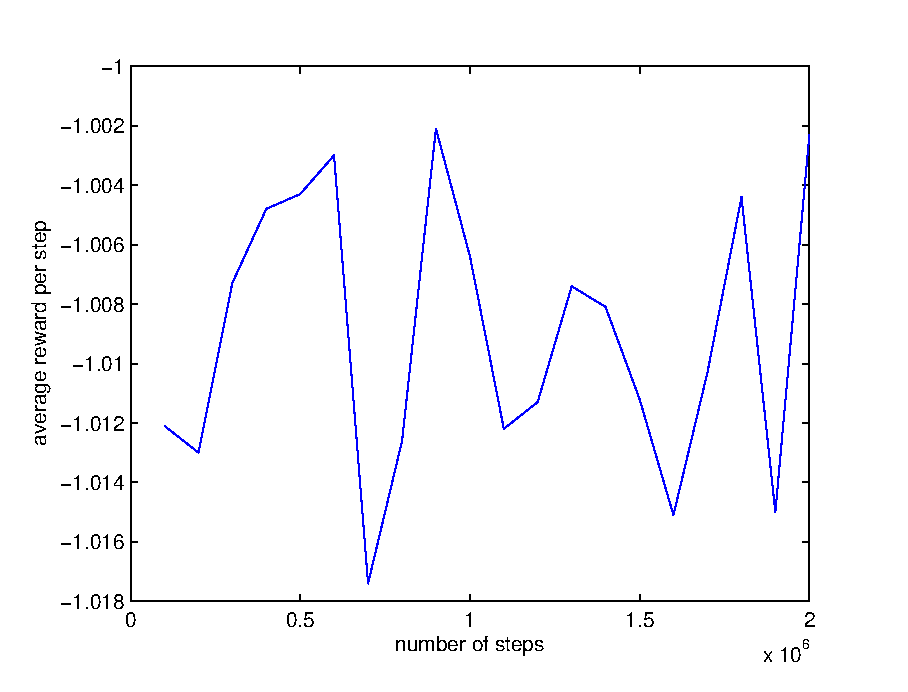
\includegraphics[width=\textwidth] {./figures/AvgReward.eps}
        %\caption{The average rewards acquired by relational template Q-Learning}
    %\label{fig:AvgReward}
    %\end{minipage}
%\end{figure}
%\begin{figure}[h]
    %\centering
    %\begin{minipage}[t]{0.48\linewidth}
        %\centering
        %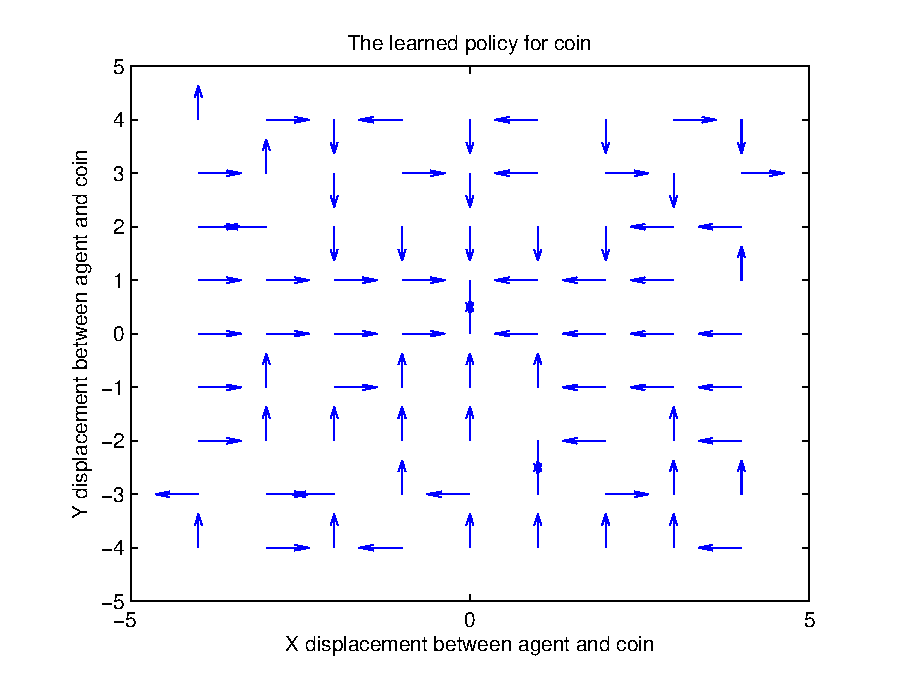
\includegraphics[width=\textwidth] {./figures/PolicyCoin.eps}
    %\end{minipage}
    %\begin{minipage}[t]{0.48\linewidth}
        %\centering
        %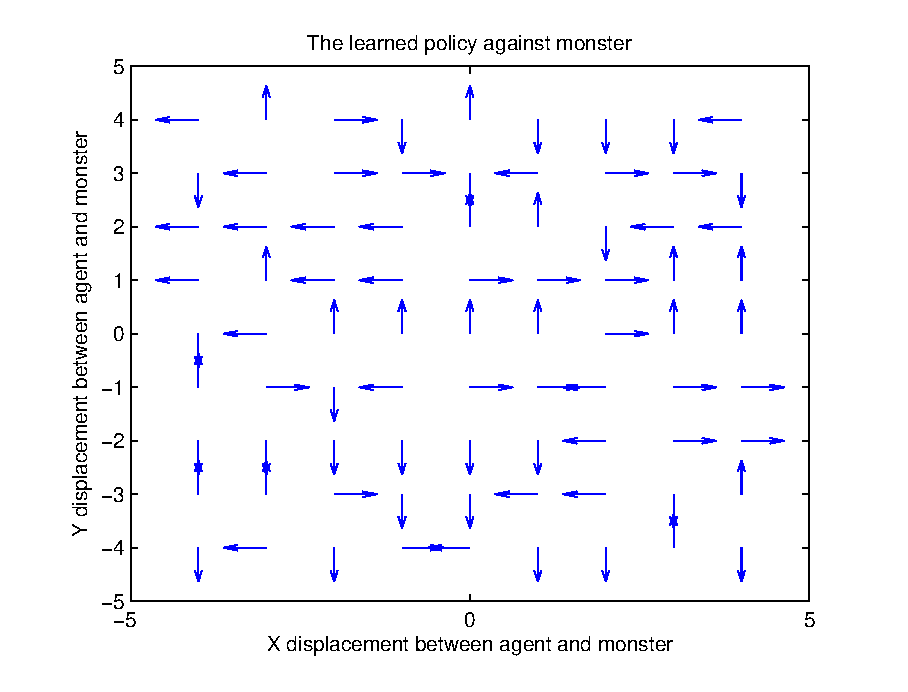
\includegraphics[width=\textwidth] {./figures/PolicyMonster.eps}
    %\end{minipage}
    %\begin{minipage}[b]{0.48\linewidth} \centering (a) \end{minipage}
    %\begin{minipage}[b]{0.48\linewidth} \centering (b) \end{minipage}
    %\caption{(a)The learned policy for a coin (b)The learned policy against a monster}
    %\label{fig:Policy}
%\end{figure}




%\section{Value Function Approximation}
%%TODO: use Literal here
%We approximate the value function as the linear combination over the basis set $h_1, h_2, \dots, h_k$, 
%where the scope of each function $h_i$ is defined by the relational features of template $t_i$.
%\[
%V(s) = sum_i w_i sum_\sigma belong I(i, s) h_i(f_{i, 1}(\sigma), \dots, f_{i, m_i}(\sigma))
%\]

%$I(trap, s) = {(A, T_1), (A, T_2)}, I(food, s) = {(A, F)}$
%$V(S) = w_{trap}(Dist(A, M_1, 1)) + V_{monster}(Dist(A, M_2, 1.4) +
%V_{coin}(Dist(A, C, 1.4))$. The local functions $V_{monster}$ and $V_{coin}$ indicates
%the expected rewards when there is one such object in the world. The
%decomposition of value function allows us to handle varying number of objects
%by summation over local functions. The class-specific local function also
%allows to share the knowledge from different objects of the same type. 
%The agent knows how to handle a new entity if the agent has experience of the same type
%before. In other worlds, the local functions enable knowledge transfer with in the 
%same class.

%\section{Relational Templates}

%The relational templates contain small number of objects of a state. 
%represent part of the states and they occur frequently and are
%relevant to the value function.

%\[
%Diff(o_1, o_2, d)
%Template_{c, c_1, c_2}(o, o_1, d_1, o_2, d_2): Diff(o, o_1, d_1) and Diff(o, o_2, d_2)
%Agent(a, o, d, o_1, d_1, o_2, d_2): Diff(a, o, d and Template(o, o_1, d_1, o_2, d_2)
%Loc(a, l) -> captures the value which is relevent to the location of the agent.
%\]

Beyond Soccer and chess. A new oppourtunituy.

Input of the program:
User cases:
1. Q-Learning
2. SARSA
3. MinMax Q
3. different parameter
4. different game (Pong, Robot Soccer, and Other)
5. different look ahead level of MinMaxQ in different games
6. Cite Sutton work
7. Cite Kevin work
8. Performance comparison of heuristic search vs RL
9. Make MinMaxQ work

Restriction of previous RL:
1. The incapability to generalize (think of an unvisited state)
2. Small number of states
3. fixed represention?

Why RL doesn't work:
dimension
example:
A MDP example with random object for each episode
(sol: Using pairwise Q function to model the Q value between agent and the object, the Q value is centered at the object and we sum it up to get the final Q function for the player)

Future:
A robot can understand how to use computer program in HCI approach


RBM:
action recognition and RL is the same: the diff is that the label of RL is an agent's action
1. heiracial can handle both space and time heiracy, and form the composition actions from the raw data
(solve 66 frames problem)
2. Can use the RBM result to reconstruct the game (how?) 
3. How to deal with dummy agent(action indepent of the env) with real agent(action depends on the env)
4. How to reuse the policy against a certain type of agent to a new unknown agent?
5. How to put the action of an agent into the hierachy? Using supervise human player video is possible, how about unsupervised?
If I can make it work, then the jitter problem of an user agent can be solved(action performed in a reduced dim, no small scale action problem anymore)
How to form a hierachical action policy?
Can use a supervised soccer video to train an agent? therefore the agent can learn the complex action automatically. (keep away soccer)
use a prior to penalize the jitter of an agent's action



6. order the objects from near to far and include the objects action in previous frame



7. the relationship between SOM
8. use different level to quantize the location of the ball and the opponent(use the past 100 frame to predict the future)
9. use different level to model the action of the players(intuition: the dim of the optimal policy is very small)
10. Question: how to create hierachical policy?
11. Iuition: the RL should be both scale and time invariant (if the movement is 0.001 pixel per frame, it should also work)
12. Model the strategy of opponent into macro action, and use them to defeat the opponent. (most video games has built-in AI, can just learn from that, 慕容復?)
If no opponent, then we have to rely on human.
13. treat action as missing data
14. intuition: the ball movement and the enemy movement are deterministic in most of the games. Therefore the dimension is pretty low.
15. For high frame rate game (like 120 FPS), it's necessary to model the opponent behavior to get the intrinsic action space
otherwise, the random walk is too slow. Or consider the Wolf 3D maze(big maze and small movement). It's too hard to rely on random walk to find the exit.
Each action replies on each expert. The switch action is equal to switch expert. (Hinton's RBM RL)
The qeustion is: when to switch the action? How to handle the big action space problem(can it be small?)
16. Cooperation ML(viki.eecs.harvald.edu)
17. curvature turning is a way to detect the boundary of an macro action (to model the opponent action)(curvature on location(x y) or action(up down left right)?)
It is better to apply it to Andrej's work on virtual avatar walking(human joint movement at walking in 1 dim)
18. create Q value from the actions in the same cluster (same scenario), combine different Q function to build a hierachy(locally trained)
19. Pong->tennis(more strategy, counter attack may fail)
20. Learning from opponent
21. MinMax SMDP Q learning
22. Copy paste programming for video games
23. Genetic algorithm from ada-boosting (you can choose different subset of training data to create different combination 
of actions)
24. collision detection as a prior information is still a way to go (pair-wise relationship modeling)
25. David: Model the transition matrix and immediate reward and use MDP instead.
26. Use convoltition to generate pairwise relationship to multipimpracticalle objects--> A Q function which centered at a block which contains 
3 objects. (spatial hierachy)
27. Fictitous gameplay with convolution. If I have pairwise model, I can simulated the game by put the player in a 
small block which contains 3 or five objects and simulated the real Q function using pairwise model.
28. The answer of taxi driver problem shall be HMM. It is nothing but first order temporal model. (each temporal
state has different task and therefore has different Q function(a function of time))
29. Convert 2D Atari games to 3D automatically (it should not be hard since you have model)(use GameMaker or 3D game studio)
30. Use spatial temporal gassian filter to distribute the rewards. The objects which are near the previous location of mario
will also get high rewards (think spatial and temporal as the same cube)(spatial and temporal proximity)
31. Use internal reward system to teach mario how to jump (if mario move to new Y loc, it gets some rewards)
32. Show the capbility to generalize the object knowledge into different stages
33. Use statistical approach to estimate which object is mario
34. Use statistical approach to estimate which objects are state object, and which objects are real world object (relieve the assumption of my work)
35. Context Free property: Expected rewards are conditional independent for different objects. Can we learn the conditionally independent partial states?
36. How to compose the different policy together?  Can “add” always work? Can we learn how to add?
37. Feature selection for reinforcement learning: Select relevant objects
38. Group lasso, how?
39. Structure Learning to find which variable is dependent on which
( use Mark Schimt approach, set weight to zero, and it remains for zero for all clusters)
Weight 0 means irrelevant. Weight 1 means disjoint, and it is default!!??

40. Group the hierachy based on sptial proximity and temporal proximity, group them toghether.
41. How to learn transition model?
42. Example of Pong in RRL, show that what RRL can do better than RL and Grid World.
43. Generalize the existing policy into unknown objects
44. Discover the same object with different appearance
45. Find the temporal proximity of a configuration.
46. Model-Based vs Model-Free approach
47. Reward distribution problem
48. Learning a policy against certain type of objects from a complex world
49. Find correct cause of the reward
45. Show how to solve MDP with model free and model-based approach. In
model-based appraoch, how to estimate the reward function.  A possible way is
to use Tzu Kuo's Master thesis to do L1 regression when some of the variables
are missing. (sol: just make it 0 for missing variables, it allows the weight
to be anything) For the constant -1 reward which does not depend on anything,
it can be regressed by Y = AX + B + e. B is the constant reward.
You can also do policy iteration by regression trees. Construct the regression tree 
by observing the neareast objects only and gradually expand the tree by adding more objects from near to far.
When there is a missing branch, it means the relation does not exists, which will also provide a value.
It is possible to have multiple branches (more than 2) for a node.

46. Init all unknown state (especiall the location of chicken)to maxV so it will encourge the chicken to walk to the other side (we don't need heirachical RL)
47. the regression approach will learn optimal state (when bullet hits a target). Any action which leads to this state will get high reward
48. RLTD, Gustrin 2003, MaxQ 2003, Russel value decomposition
49. Call this paper: relational template selection and claim novelty and effectiveness against TD-RRL
50. the relationship with Peter Stone's Robot Soccer, experiment on Robot Soccer
51. Experiment on L2 regularization and L1 and no regularization
52. agent location detection
53. threat detection: locate the most threaten objects in screen (it may or may not be nearest one)
54. You can only use VMAX for lower level model (why?)
55. Do you need to seperate different rewards?
56. You need to scale the rewards to [-1, 1], or you need to adjust regularization constant everytime, also, the real weight should fall in [-1, 1]
57. Use forward feature selection from lower order model to higher order and exclude the higher order variable if the lower order model is excluded
58. Use group lasso to select the location of agents.
59. Use different regularization term. regularize higher order predicate heavier? massage the regularization term???
60. Use monte carlo sampling to sample the world in keepaway soccer
61. Show that 3vs2 keepaway to 4vs3 is unneccessary and harmful. You should use 2vs1 to 4vs3. (motivate the necessity to use progressive transfer learning)
62. transfer directly from 2vs 1 to 10vs9
63. Show that without higher order predicate, it's not useful to train in high order scenario, and it can also be harmful
64. Show higher order predicate is useful, but the effect will die away
65. Show progressive learning will outperform any learning in single scenario (1 vs 1 + 2 vs 2 > 2 vs 2), use the same 10 sec criteria
66. Scale up to 9 vs 10
67. The motivation: the real predicates are unknown, you need a way to find true related template. Write it in the perspective of relational templates.
68. Compare with RLTD
69. Relational View of keepaway soccer
70. Show that the common prototype of video games like Raiden or Ys have finite size of relational template(Higher order of templates will vanish)
71. RL is all about finding the shortest path to the reward. I can use model based approach. Build a movement model without object.
    Build a reward model without object. Then put objects one by one, build more complex models. The value function
    can be computed by the weighted shortest path algorithm.
72. Use hard-coded agent to sample and tell the ptl which feature is relevant
73. Use the distrution which has long tail on the left but not on the right as the prior of the sample Q values, put a lot of confidence on the prior unless the sample points are really really huge
74. Why RL? because it can handle unoberserved event--> an invisible wall in the dungeon. Or a false wall.
75. Backtracking how?
76. Technique: 1.learning from simpler scenario (linear SARSA doesn't work) 2. search(back tracking)(linear SARSA doesn't work)
77. Technique (no simulation environment, game mechanism is not fully understood, too complex):
    1. learning from hand-coded agents and optimize it--> 
       1.1. purly use it as exploration policy and update the Q function
       1.2. use its feature selection as additional information and pretend the agent is learning in the simplified scenario (useful if we need to play simplified scenario later--> works if there are many objects of the same kind, which is very noisy)
    2. learning from human player
































\chapter{Relational Reinforcement Learning for Keepaway Soccer}


\section{Experiment}

\begin{figure}[h]
    \centering
    \begin{minipage}[t]{0.6\linewidth}
        \centering
        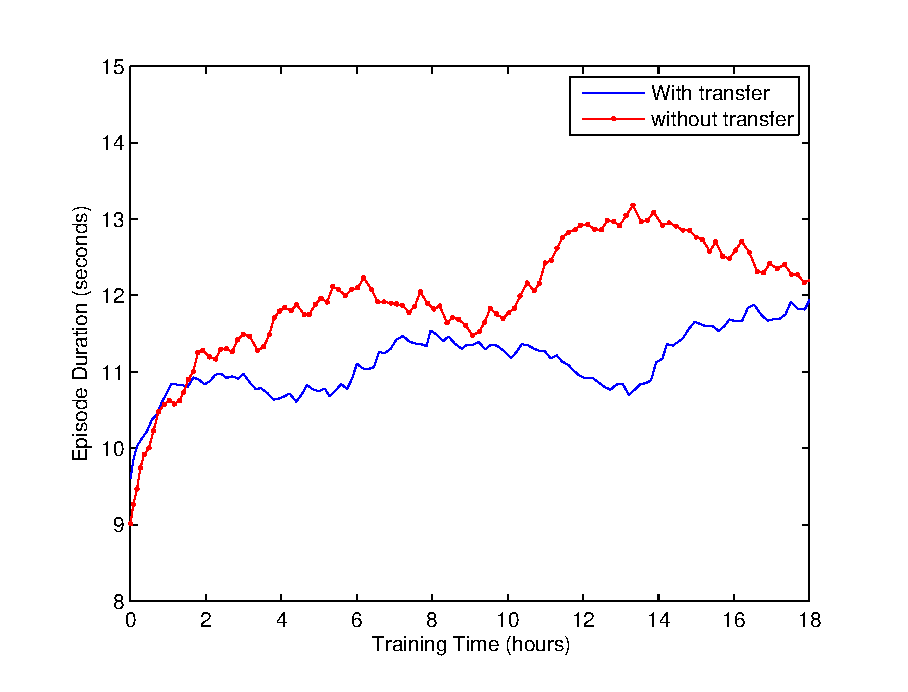
\includegraphics[width=\textwidth] {./figures/3vs2transfer.eps}
        \caption{The learning result of 3 vs 2 keepaway with/without prior training}
    \label{fig:3vs2transfer}
    \end{minipage}
\end{figure}

\begin{figure}[h]
    \centering
    \begin{minipage}[t]{0.6\linewidth}
        \centering
        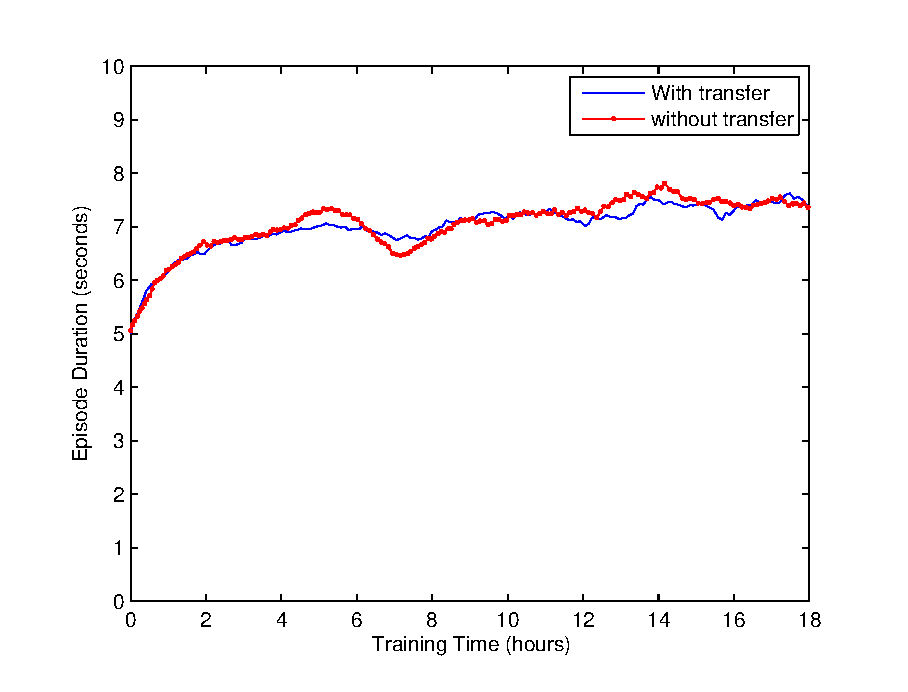
\includegraphics[width=\textwidth] {./figures/4vs3transfer.eps}
        \caption{The learning result of 4 vs 3 keepaway with/without prior training}
    \label{fig:4vs3transfer}
    \end{minipage}
\end{figure}

The experiment is performed in keepaway soccer simulator available at \\
(\url{http://www.cs.utexas.edu/~AustinVilla/sim/keepaway/}).
We first run the $SARSA(\lambda)$ to the 3 vs 2 keepaway soccer with all weights initialized to the highest possible reward (optimistic exploration). The exploration policy is 
the $\epsilon-greedy$ with $\epsilon$ set to 0.01. The temporal different coefficient $\alpha$ is set to 0.125 and the 
discount factor $\gamma$ is 0.95. The field size of the keepaway soccer is $20 \times 20$. 
The result is shown in Fig. \ref{fig:3vs2transfer} and \ref{fig:4vs3transfer}. 

To test our hypothesis, we then trained the agent in 1 vs 1 keepaway soccer for 200 episodes. 
In this simple scenario, the agent has no teammates, therefore the only action available to it is to hold the ball.
It helps the agent to learn the correct value for holding the ball all the times.
Clearly, the training of 1 vs 1 scenario is not enough for the agent to succeed since it does not know
when to pass the ball to its teammate. As a result, we use the knowledge of 1 vs 1 scenario as prior knowledge, 
and further trained it in 2 vs 1 keepaway for 1000 episodes.
With the knowledge about the 1 vs 1 and 2 vs 1 scenarios, the agent now can do better in 3 vs 2 and 4 vs 3 keepaway (Fig. \ref{fig:3vs2transfer} and \ref{fig:4vs3transfer})
than the untrained one.

\section{}
\[
   P(w, \mu, \Sigma| D) = P(D|\mu, \Sigma)P(\mu|w^Tu, I)P(w)\\
   P(w, \mu, \Sigma, h| D) = P(D|\mu, \Sigma)P(\mu|w^Tu, I)P(w|h)P(h)\\
   P(w, \mu, \Sigma, h| D) = P(D|\mu, \Sigma)P(\mu|h, I)\\
\]





























%\include{impl}
%\chapter{Conclusions}

%Our result suggests the possibility incorporating a wide range of planning
%techniques such as STRIPS [11] or object-oriented RL [16] into the HRL framework without the
%loss of optimality. One future direction is to investigate the applicability of combining our method
%with such techniques.

Model-based methods are powerful tools. It allows us to predict the outcome 
of the agent behavior and plan over it. They can effectively reduce the number of 
samples which are required to find the optimal policy.
However, model-based methods may not be able to learn the optimal
policy due to the structural assumptions.
%However, model-based methods may not be able to learn the transition function correctly.
%The possible reasons are:
%\begin{itemize}
%\item The inaccuracy in the supervised learning algorithms
%\item The numerical imprecision in the continuous case
%\item It is not possible to learn all the effects
%\item It would be time-consuming if we compute all possible effects during planning process
%\end{itemize}
In this work, we propose an approach to combine the approximate model-based method with the
model-free method (HORDQ) under the HRL framework. We are able to show that our approach
can learn the optimal policy even when the assumption of model is not satisfied. Furthermore, we show that the optimality
is guaranteed for any subtask policy as long as the subtask does not belong to the total leaf
cover of given hierarchy.

In this chapter, we share our experience about how to apply our theory to design a system.
Since the performance of system highly depends on the value of pseudo-reward, we will also introduce
some heuristics for choosing an appropriate pseudo-reward.
Finally, we discuss the limitation and possible future works of our theory. 

%In this thesis, we describe an approach to use model-free methods to 
%compensate the scenarios when model-based methods are failed to learn the optimal policy.
%In small problems which we can use table-lookup methods, it is guaranteed to learn the optimal
%policy. 
%For large problems, there are no guarantee, but we should 
%The choice of features of model-free methods effect the overall performance
%If we put too much irrelevant features, the qualify of learned policy will be severed.

\section{System design}

An important design principle of the system is to design the model-based method first,
and the model-free method later. 
We need to decide the features used by the
model-based methods, the underlying supervised learning algorithms and most
importantly, the effects which we would like to include in our model. Then we
run the experiments, and observe the scenarios where the model-based method
is failed. 
Based on the observations, we design a set of features for model-free methods to handle
these scenarios. Note that we don't need to design a set of features to handle
the whole problems, but only part of it. We only need the model-free method
to take control when the model-based method fails. Therefore, we can reduce the
number of features for model-free methods and let the overall system
successfully handle all scenarios.

%//There are other alternative approaches to overcome their limitation.
Since our work is about how to use model-free methods to improve the learned policy of model-based methods,
it is not necessary to adopt our work if model-based methods can learn the optimal policy
on their own.

Our work is not the only solution when model-based methods fail.
Another alternative is to improve the quality of the model by including more domain knowledge.
For example, in our Infinite Mario experiment, we do not include any effects 
of the interactions between monsters and Mario. It is possible to
hand-code the preconditions and postconditions of these effects, as Walsh et al. proposed in \cite{Walsh09}.
In fact, the source code of Infinite Mario is publicly available.
%(TODO: source code)
There are no need to use model-based methods to learn the model. Instead,
we can simulate the experiences of the agent with the simulator of Infinite Mario. 
Since the environment and the model are identical, there are no biases which will be 
introduced during the simulation process.
It is what Baumgarten did with his $A^*$ method for Mario AI\cite{Robin09}.
With the complete domain knowledge, it is unlikely for any RL methods to outperform his work.

However, the key idea of RL is to build an adaptive agent.
Not only do we want the agent to perform well in a problem which we know very well,
but we also want the agent to adapt itself to novel problems which we cannot foresee when we design the agent.
If we put too much domain knowledge into the agent's design, we forbids it from adapting 
itself when the prior knowledge does not hold anymore. 
In this work, we introduce an alternative -- instead of designing an omnipotent model-based agent, we
divide the learning task into different parts and let model-free methods handle the parts which model-based methods cannot do.

%We want the agent to adapt itself to novel scenarios and find the optimal policy.
%If we put too much domain knowledge into the design of the model, the agent 
%will not be able to adapt when the knowledge does not hold in these scenarios.
%If we put too less, the model may be poor-approximated, 
%and hinder the learning process. 
%(TODO: my school bus exp)
%Our work tries to find a balance between 


%TODO: relationship with HRL (no 
%Although we use HRL framework to incorporate model-based and model-free methods, 
%TODO: the choice of model-free methods (not only HORDQ), anything that can know its consquences  
%It is not a problem to find a hierarchy

\section{Choose an appropriate pseudo-reward}
It is important to choose an appropriate pseudo-reward. If we choose a pseudo-reward which is too small, 
the policy of the agent will be similar to the policy of model-free method. Therefore, we may lose the 
benefit of faster learning rate. On the other hand, if the pseudo-reward is too large, 
the policy will be similar to the model-model method, which may be suboptimal
when the assumptions of the model are not all satisfied.

It is easy to determine when a pseudo-reward is too large by
looking at the difference between the expected reward of the optimal policy and the policy of model-based method.
If a pseudo-reward is larger than the difference, the model-free method will follow the policy
of the model-based method strictly, and the combined policy will be the same as 
the policy of model-based method.

In our experiments (Sections \ref{se:BusRes} and \ref{se:MarioRes}), a pseudo-reward larger than the expected death penalty is considered "too large", 
since it will let the model-free method follow the instruction of model-based method even 
when it will result in the death of the agent. If we choose a pseudo-reward which is smaller than it,
the model-free method will choose an action that avoids the death of the agent.

It is more difficult to decide if the pseudo-reward is large enough. 
For small problems, if we adopt table-lookup HORDQ as the model-free method,
the optimal policy will be learned when the pseudo-reward is decreased to zero.
So a viable strategy is to choose some pseudo-reward, which is not too large, and
gradually decrease it to zero.
For large problems, we have adopt model-free methods with function approximation techniques
, therefore the optimal policy might not be learned when the pseudo-reward is zero.
Instead, we need to find out an optimal pseudo-reward which can maximize the expected reward.
A way to decide it is to conduct the experiment with the model-free method,
and choose a pseudo-reward which is large enough to encourage
the model-free method to follow the policy of model-based one.
%It is necessary to have a large pseudo-reward in the beginning since 
%the model-based method does not have enough samples to build a good model,
%it is possible for it to compute very poor policy.

\section{Limitation and future work}

The quality of learned policy depends on the chosen model-free method,
the model-based method and the pseudo-reward. 
Since we can control the pseudo-reward to decide if the combined
policy should be similar to model-free or model-based one,
the combined policy can never be worse than any of them. 

Since our work is a combination of two,  Our work will fail in scenarios where both methods fail, 
It is only possible to resolve it by applying better model-free or model-based methods. 

%If we adopt the task hierarchy in \ref{se:MarioExp}, we can apply our work
%to any reinforcement learning problems.  
%The limitation of the applicability
%of our work actually comes from the underlying RL methods. 

Nevertheless, our work is not be useful when one method outperforms another.
In general, model-based methods learn faster than model-free methods because of
efficient use of samples, but it may not be true for some problems. 
If the chosen model-based method is worse than the model-free method in both learning
rate and the learned policy, it is pointless to combine both methods. 
Similarly, if the model-free method fails to handle the scenarios where the model-based
method fails or the model-based method can learn the optimal policy, it is not necessary to apply our work.
For small problems, if the model-based method fails to learn the optimal policy, 
we learn the optimal policy by combining it with table-lookup HORDQ as we prove in Theorem \ref{thm:opt}.
For large problems, it is difficult since approximated model-free RL may not learn the optimal policy.
It is necessary to have the knowledge about the domain and apply the knowledge to choose some good features.

%TODO: the process is similar to model-free RL
We introduced the theory of improving the quality of the policy of model-based methods. However, we don't have any theory regarding the learning rate.
It is true that if the model-based method is "approximately good", we can enjoy the 
faster learning rate, as we showed in the experiment of Bus domain. Nevertheless, there are no theory
to tell if a model-based method is approximately good or not.
A possible direction of future work is to investigate what kind of the properties of model-based
methods are necessary to increase the learning rate and how much they can increase when they are combined with model-free methods.




%1. No theory about learning rate (what is a good approximation?)
%2. No thery about the interaction betwwen model-based and model-free approach.
%If model-base dapproahc does not change it's policy accroding to model-free's policy,
%the learning can be slower than pure model-free. Since model-based method
%will stick on it's original bad plan, and guid the agent to the wrong action.

%A problem may arise when the pseudo-reward is 

%The performance of our approach depends on 
%Large enough so that the model-free approach will pursue the subgoal
%When the model-based approach doesn’t have enough samples to build an approximately good model
%Small enough to pass the control to model-free approach when the model-based approach doesn’t work

%Combine both model-free and model-based approaches
%Overcome the structure assumption of model-based approaches
%Learns a better policy by mixing these approaches
%Designing pseudo-reward requires insight of the problem
%No theory yet!

%model-based or model-free is too good

%We have presented a learning algorithm for agile, integrated whole-body
%skills of physically-simulated characters. The algorithm uses a nature-inspired
%online, active exploration of the character action space to nd reliable mo-
%tions that give rise to parameterized skills. We further demonstrated that
%our algorithm works for a family of simple characters without requiring any
%algorithm or parameter modications. In addition, we experimented with
%a complex dog character in 3-D and showed that our approach generalizes
%to this character, given appropriate changes in the motor abstractions used
%during the learning process. Finally, we showed that the resulting parame-
%a terrain.
%5.1 Discussion
%While a learning approach to acquiring skills possesses many benets, it also
%comes with its own set of limitations.
%Mainly, we found that the learning process requires occasional super-
%vision to ensure that the intended skills are actually being learned. For
%example in one case, a character learned a Flip motion that made it launch
%necessary to supervise the learning process and restart it on a few occasions.
%The majority of skill and character combinations (roughly 90%) did not re-
%quire any interventions. We believe that these issues could be alleviated by
%better quantifying when a particular trial should count as being successful

%for every skill.
%In addition, the phase 1 reward functions may be dicult to specify in
%some cases. In particular, we found the GetUp skill to be the most trou-
%blesome. If the character fails at getting up after some Motor Action, how
%should one assign a score for how close the attempt was? Specifying a bad
%phase 1 reward function could lead to long computation times in phase 1,
%because the character is essentially left searching randomly in the motor
%space for a successful action. Even worse, the optimization in phase 1 could
%be repeatedly led astray with an inappropriately specied phase 1 reward
%function.
%The main challenges for the quadruped character were aesthetic in na-
%ture. Unlike the Acrobot's motions, a dog's leap is a specic type of motion
%that we are all familiar with from nature. Even though the learning al-
%gorithm produced leaps that accomplished all desired goals, they did not
%always resemble leaps that one would expect to see from a real dog. For
%but this motion did not emerge in the actions that were produced by the
%algorithm. Instead, the dog left its front feet outstretched during the leap,
%producing a motion that felt qualitatively strange despite achieving all task
%goals. In the end, we opted to include these details into the leap controller
%manually to achieve a more familiar style of motion.
%5.2 Limitations and future work
%Even though the learning algorithm described in this thesis works well for
%our characters and the set of skills we considered, we make no claims to
%have addressed the general problem of motor learning. In this section, we
%discuss possible extensions of the proposed framework that can bring us
%closer toward the nal goal of matching human or animal abilities.
%To begin with, several immediate improvements can be made to the
%framework by addressing some of the simplications that were made mostly


%\include{conclusions}

%    3. Notes
%    4. Footnotes

%    5. Bibliography
\begin{singlespace}
\raggedright
\bibliographystyle{abbrvnat}
\bibliography{biblio}
\end{singlespace}

\appendix
%    6. Appendices (including copies of all required UBC Research
%       Ethics Board's Certificates of Approval)
%\include{reb-coa}	% pdfpages is useful here

\backmatter
%    7. Index
% See the makeindex package: the following page provides a quick overview
% <http://www.image.ufl.edu/help/latex/latex_indexes.shtml>


\end{document}
